\documentclass{article}
\usepackage[a4paper,hmargin=2cm,top=2.25cm,bottom=3cm]{geometry}
\usepackage{graphicx} % Required for inserting images

\usepackage{url}
\bibliographystyle{apalike}
\usepackage{hyperref}
\usepackage[table,xcdraw]{xcolor}
\usepackage{fancyvrb}
\usepackage{minted}
\usepackage{amsmath}
\usepackage{cleveref}
\usepackage{subcaption}
\usepackage{dirtytalk}
\usepackage{parskip}
\usepackage{colortbl} 
\usepackage{multirow}
\usepackage{booktabs}
\usepackage{multicol}
\usepackage{makecell}

\usepackage{cleveref}
\usepackage{verbatim}
\usepackage{appendix}
\usepackage{listings}
\usepackage{amsfonts,amsthm}
\usepackage{tikz}
\usetikzlibrary{positioning,shapes,arrows}
\lstset{breaklines=true, basicstyle=\ttfamily}

\setlength\parskip{2ex plus 0.2ex minus 0.4ex}
\setlength\parindent{0em}

\DeclareCaptionSubType[alph]{listing}



% \title{PAR Exercise 1. Mining Robot Task.}
% \author{Andreu Garcies Ramon\\Maria Guasch Torres}
% \date{October 2025}

\title{
    \textbf{A1: Structural descriptors of complex networks}\\
    \large Complex Networks\\
    \small Universitat Rovira i Virgili (URV)\\
    \small Master in Artificial Intelligence (MAI)
}
\author{
    Andreu Garcies Ramon\\
    \texttt{andreu.garcies@estudiantat.upc.edu}
    \and
    Maria Guasch Torres\\
    \texttt{maria.guasch.t@estudiantat.upc.edu}
}
\date{March 2026}

% \bibliographystyle{apa}

\begin{document}


\maketitle

\section{Introduction}

The goal of this report is to present the analysis of the results obtained for the first assignment of the subject. It analyzes the structural properties and the underlying models of different complex networks. To achieve this, a set of macriscopic and microscopic descriptors are used to characterize both the global topology of the networks and the role of some individual nodes within them. Based on these properties, each network is then associated with a well-known model, including Watts-Strogartz, Erdös-Rényi, Configuration Model, and the Barabási-Albert. Finally, an additional network is studied, for which an algorithm that could have generated it is also proposed.


\section{Part 1: Structural Characterization of networks}\label{sec:part1}

% In this section we analyze several network descriptors for four different networks.

% \subsection{Metrics} % maria

In order to characterize the four synthetic networks studied in this activity, we first establish a set of network descriptors. These metrics allow us to quantify both the global topology of the network (macroscopic structure) and the individual importance of its nodes (microscopic structure). 

\subsection{Macroscopic descriptors: overall network structure}

To assess the global properties of each network, we calculate the following macroscopic metrics:

\begin{itemize}
    \item \textbf{Number of nodes $N$ and edges $K$:} These two values define the basic size of the network.
    \item \textbf{Node degree ($k$):} The degree of a node represents the number of edges which are connected to it. Particularly, we analyze the minimum, maximum and average degree $\langle k \rangle$ of the network to understand its general connectivity.
    \item \textbf{Average clustering coefficient $\langle CC \rangle$:} This metric measures the local cohesiveness of the network. That is, it represents the average probability that two neighbours of a particular node are also connected to each other, forming a triangle. 
    \item \textbf{Degree assortativity $r$:} It measures the tendency of nodes of degree $k$ to connect to nodes of degree $k'$. It is the correlation coefficient of the degrees between pairs of nodes that are connected by an edge. A high assortativity value indicates that high degree nodes are likely connected to other high degree nodes (hubs), while a low value (a dissassortative network) indicates that high degree nodes tend to connect to low degree nodes.
    \item \textbf{Average path length $\langle l \rangle$:} This is the average number of links that compose a path connecting two nodes in the network.
    \item \textbf{Diameter $D$:} The diameter represents the maximum shortest path length found in the network.
\end{itemize}

\subsection{Macroscopic analysis}


\begin{table}[h]
\centering
\begin{tabular}{lcccc}
\toprule
\textbf{Metric} & \textbf{net1} & \textbf{net2} & \textbf{net3} & \textbf{net4} \\
\midrule
Number of nodes & 5000 & 5000 & 5000 & 5000 \\
Number of edges & 25000 & 24873 & 23508 & 24975 \\
Max degree & 16 & 24 & 732 & 210 \\
Min degree & 6 & 1 & 3 & 5 \\
Average degree & 10.0 & 9.9492 & 9.4032 & 9.99 \\
Avg. clustering coefficient & 0.4141 & 0.0021 & 0.0862 & 0.0107 \\
Degree assortativity & -0.0097 & -0.0057 & -0.1339 & -0.0325 \\
Avg. shortest path length & 5.1211 & 3.9560 & 3.0082 & 3.4868 \\
Diameter & 8 & 7 & 5 & 5 \\
\bottomrule
\end{tabular}
\caption{Structural characterization of the four analyzed networks.}
\label{tab:network_characterization}
\end{table}

The results of computing these macroscopic metrics on the four provided networks are summarized in Table~\ref{tab:network_characterization}. The four networks share the same macroscopic size, at exactly $N=5000$ and approximately 25000 edges each, resulting in an average degree $\langle k \rangle$ of around 10 for all of them. However, the remaining structural descriptors vary from network to network, revealing their underlying topologies.

A key difference among the networks is their degree heterogeneity. Networks \textit{net1} and \textit{net2} show highly homogeneous structures, as their maximum degrees (16 and 24, respectively) remain close to the network average. This would indicate that edges are evenly distributed among all the nodes in the network. However, \textit{net3} and \textit{net4} show maximum degrees of 732 and 210, which are more extreme values. These highly connected hubs, along with low minimum degrees, suggest a heavy-tailed degree distribution where a few massive hubs coexist with a large majority of poorly connected peripheral nodes.

\begin{figure}[htbp]
    \centering
    % --- First row ---
    \begin{subfigure}[b]{0.45\textwidth}
        \centering
        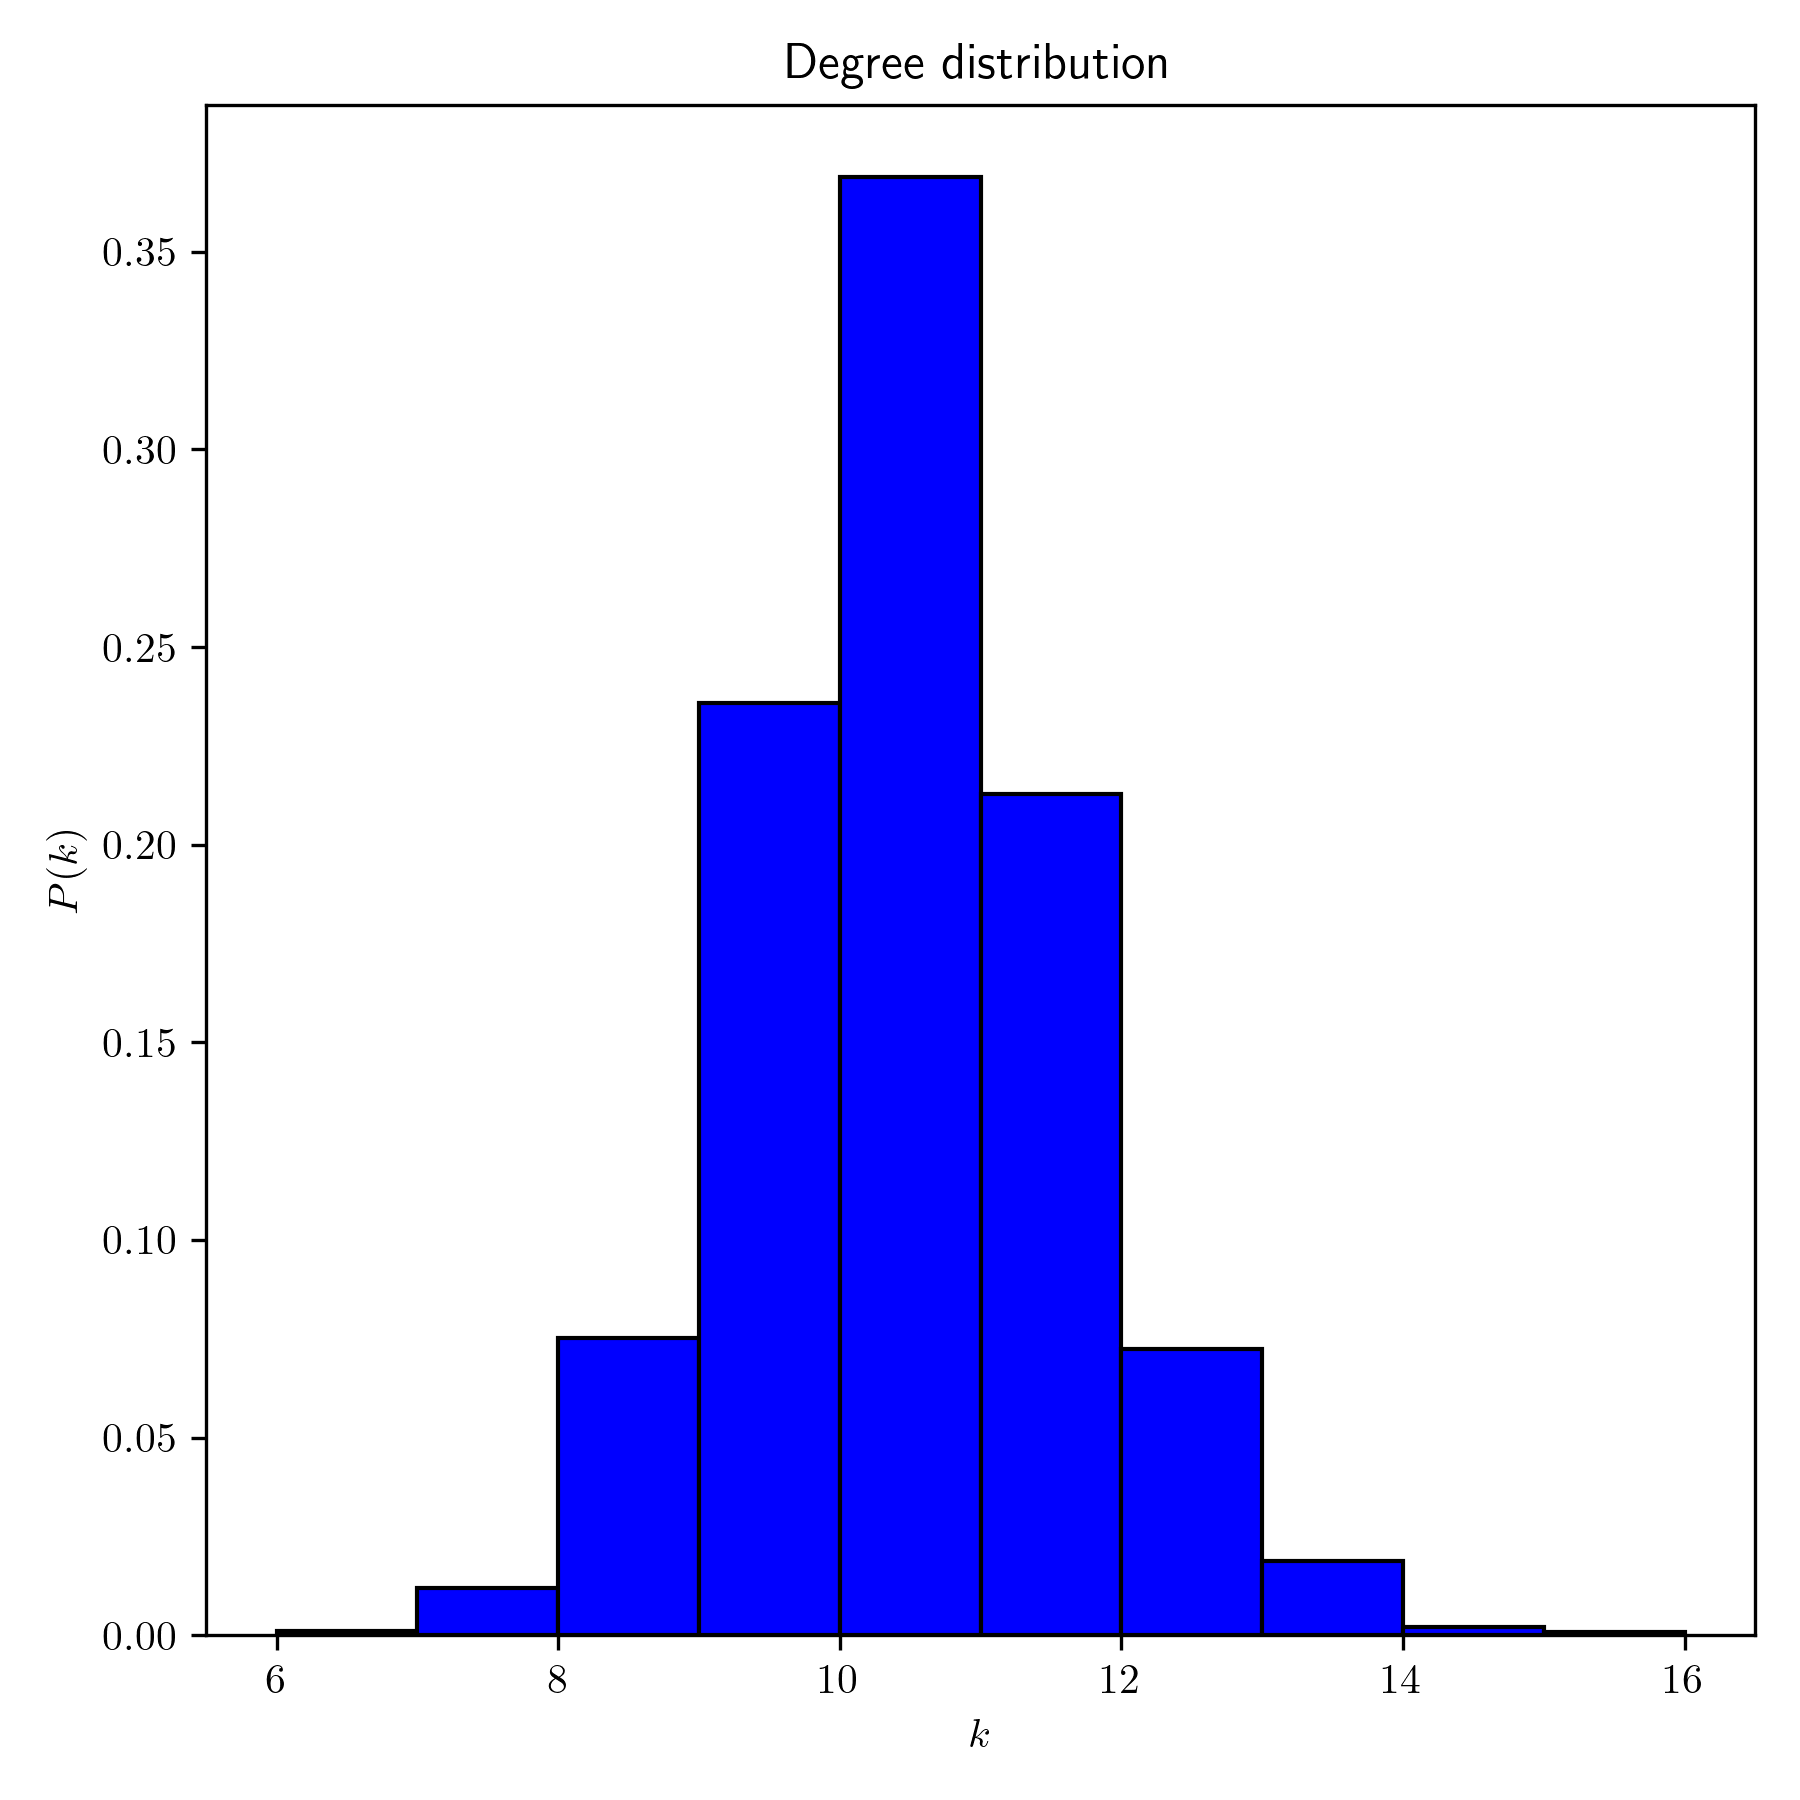
\includegraphics[width=\textwidth]{assets/net1net_hist.png}
        \caption{Degree distribution of \textit{net1}}
        \label{fig:net1_hist}
    \end{subfigure}
    \hfill
    \begin{subfigure}[b]{0.45\textwidth}
        \centering
        
\includegraphics[width=\textwidth]{assets/net2net_hist.png}
        \caption{Degree distribution of \textit{net2}}
        \label{fig:net2_hist}
    \end{subfigure}
    
    \vspace{0.5cm} 
    
    % --- Second row ---
    \begin{subfigure}[b]{0.45\textwidth}
        \centering
        
\includegraphics[width=\textwidth]{assets/net3net_hist.png}
        \caption{Degree distribution of \textit{net3}}
        \label{fig:net3_hist}
    \end{subfigure}
    \hfill
    \begin{subfigure}[b]{0.45\textwidth}
        \centering
        
\includegraphics[width=\textwidth]{assets/net4net_hist.png}
        \caption{Degree distribution of \textit{net4}}
        \label{fig:net4_hist}
    \end{subfigure}
    
    \caption{Degree distributions for the four networks (linear scale, linear binning).}
    \label{fig:degree_distributions}
\end{figure}

Figure~\ref{fig:degree_distributions} provides a more detailed view of the node degree distributions. Both \textit{net1} and \textit{net2} present rather homogeneous degree distributions, resembling a Gaussian or Poisson bell curve. Since their maximum degrees are close to the average, we can infer that these networks do not contain large hubs, which aligns with our earlier analysis. However, \textit{net3} and \textit{net4} display much more heavy-tailed distributions. In these cases, the majority of nodes have a low degree, while just a few of them have a higher number of edges.

\begin{figure}[htbp]
    \centering
    % Row 1
    \begin{subfigure}[b]{0.45\textwidth}
        \centering
        
\includegraphics[width=\textwidth]{assets/net3net_hist.png}
        \caption{Standard Histogram}
        \label{subfig:net3_hist}
    \end{subfigure}
    \hfill
    \begin{subfigure}[b]{0.45\textwidth}
        \centering
        
\includegraphics[width=\textwidth]{assets/net3net_hist_log.png}
        \caption{Log-Scaled Histogram}
        \label{subfig:net3_hist_log}
    \end{subfigure}
    
    \vspace{1em} % Adds vertical space between rows
    
    % Row 2
    \begin{subfigure}[b]{0.45\textwidth}
        \centering
        
\includegraphics[width=\textwidth]{assets/net3net_hist_logbin.png}
        \caption{Log-Binned Histogram}
        \label{subfig:net3_hist_logbin}
    \end{subfigure}
    \hfill
    \begin{subfigure}[b]{0.45\textwidth}
        \centering
        
\includegraphics[width=\textwidth]{assets/net3net_ccdf.png}
        \caption{Degree CCDF (Log-Log Scale)}
        \label{subfig:net3_ccdf}
    \end{subfigure}
    
    \caption{Degree distribution analysis of \textit{net3}. 
    }
    \label{fig:net3_distributions}
\end{figure}

\begin{figure}[htbp]
    \centering
    % Row 1
    \begin{subfigure}[b]{0.45\textwidth}
        \centering
        
\includegraphics[width=\textwidth]{assets/net4net_hist.png}
        \caption{Standard Histogram}
        \label{subfig:net4_hist}
    \end{subfigure}
    \hfill
    \begin{subfigure}[b]{0.45\textwidth}
        \centering
        
\includegraphics[width=\textwidth]{assets/net4net_hist_log.png}
        \caption{Log-Scaled Histogram}
        \label{subfig:net4_hist_log}
    \end{subfigure}
    
    \vspace{1em}
    
    % Row 2
    \begin{subfigure}[b]{0.45\textwidth}
        \centering
        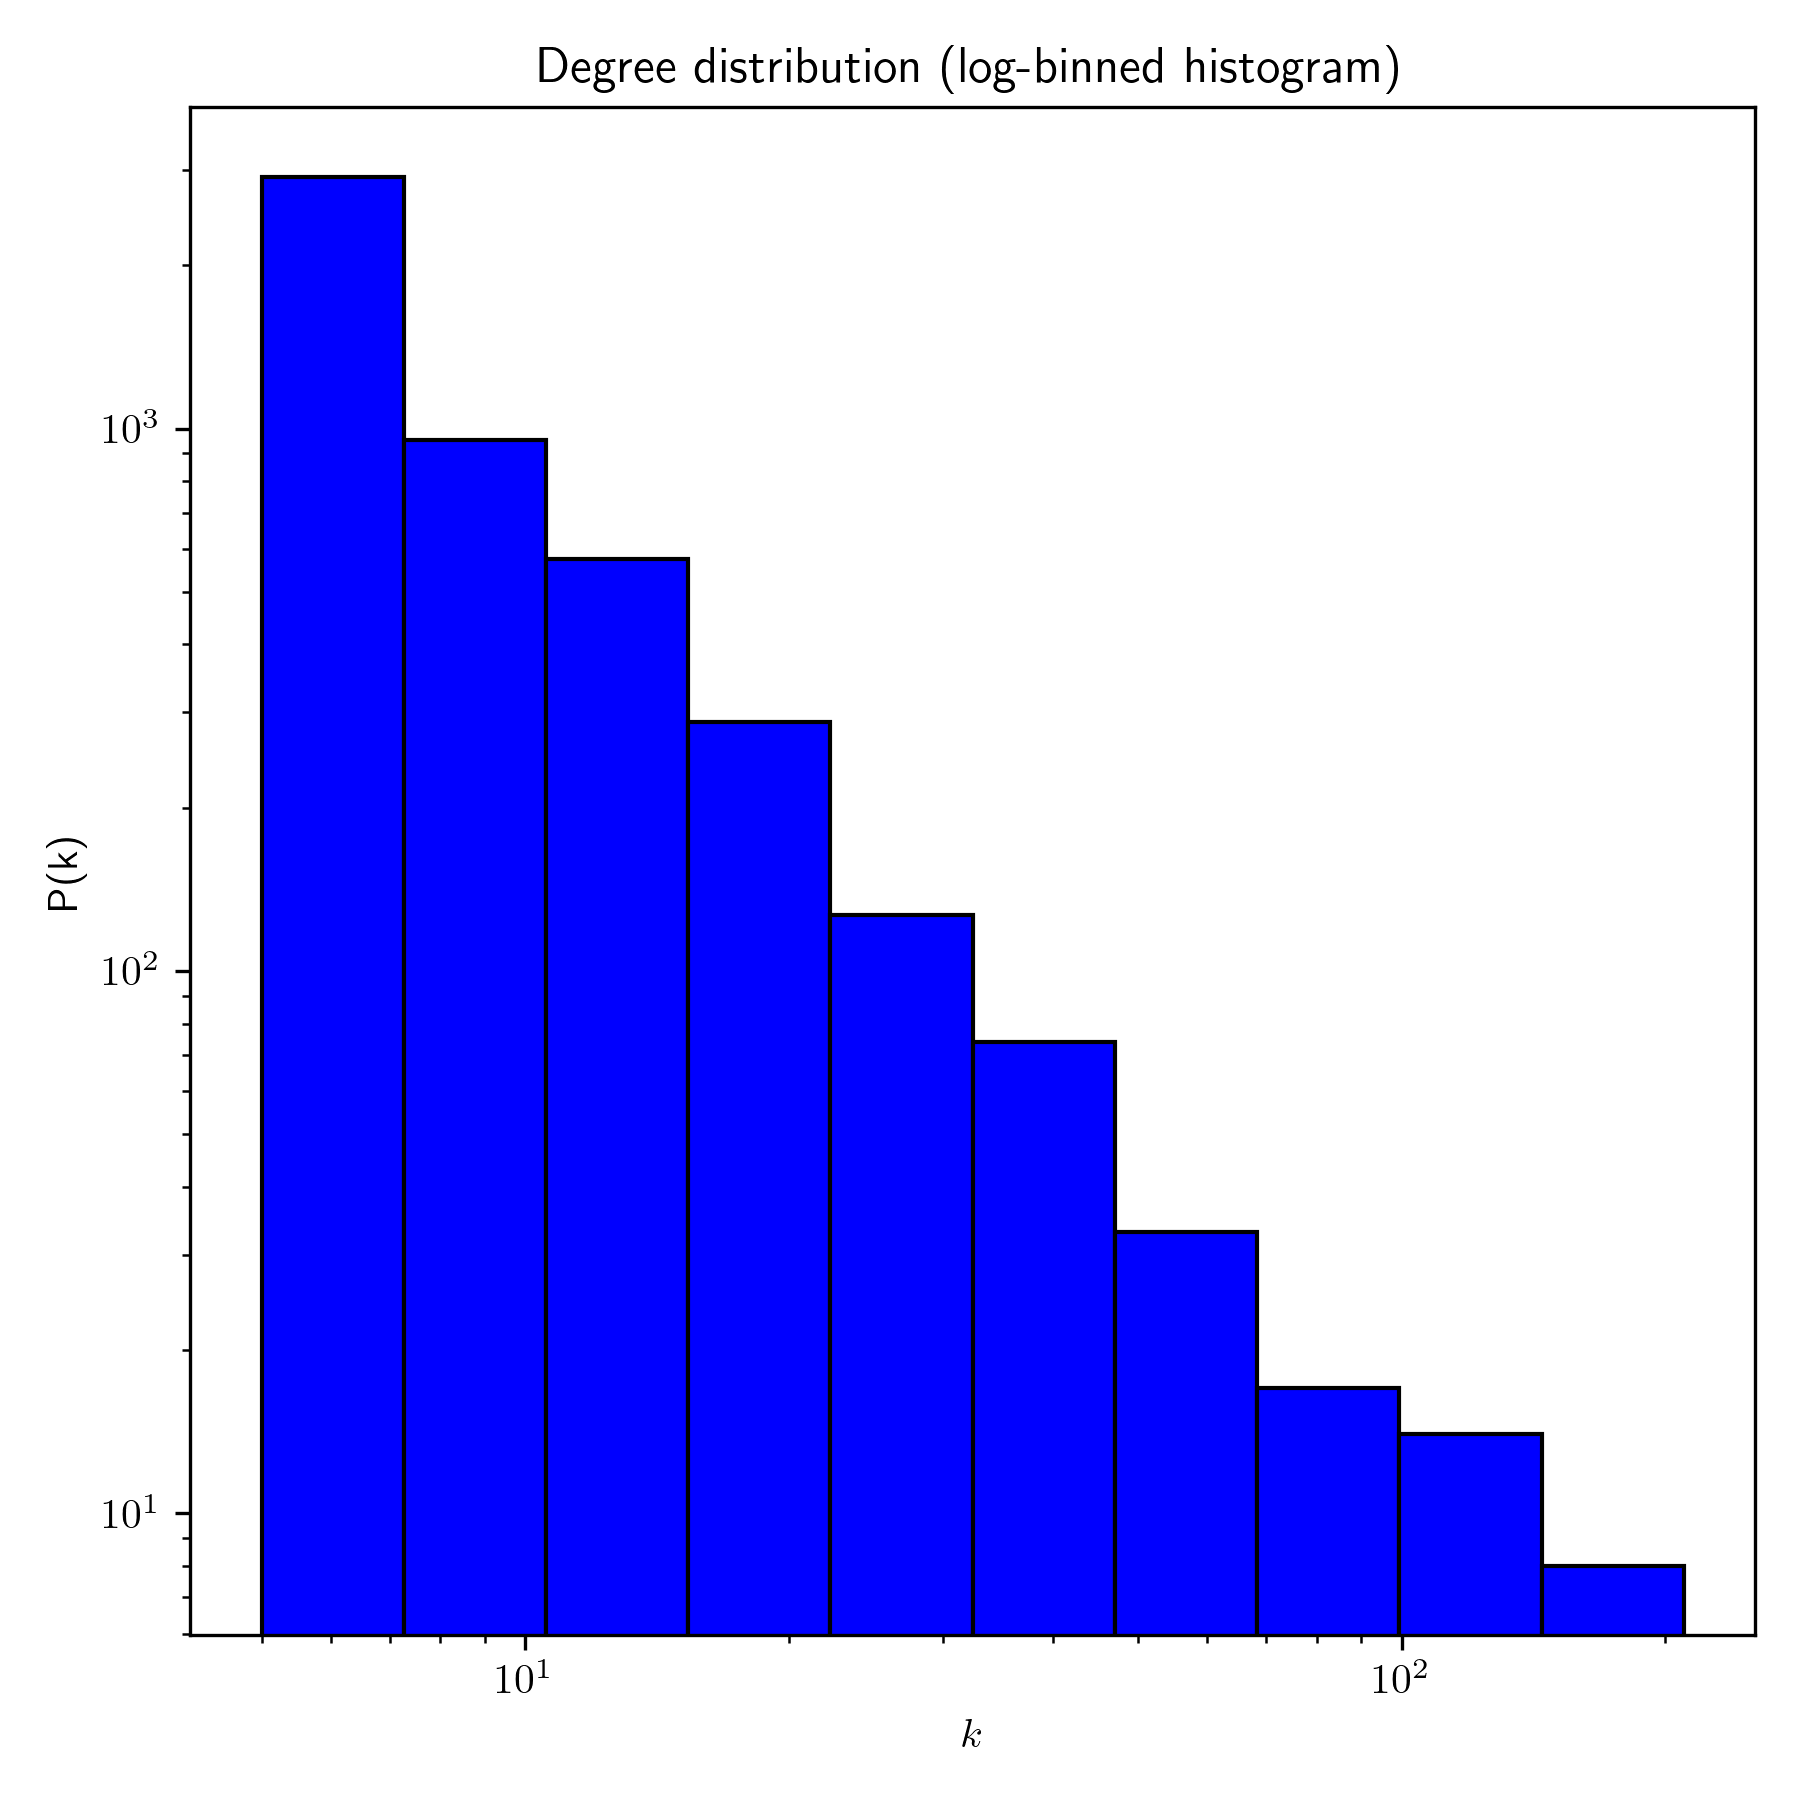
\includegraphics[width=\textwidth]{assets/net4net_hist_logbin.png}
        \caption{Log-Binned Histogram}
        \label{subfig:net4_hist_logbin}
    \end{subfigure}
    \hfill
    \begin{subfigure}[b]{0.45\textwidth}
        \centering
        
\includegraphics[width=\textwidth]{assets/net4net_ccdf.png}
        \caption{Degree CCDF (Log-Log Scale)}
        \label{subfig:net4_ccdf}
    \end{subfigure}
    
    \caption{Degree distribution analysis of \textit{net4}. 
    % Similar to \textit{net3}, the progression from the standard histogram (a) to the log-binned plots (b, c) illustrates a heavy-tailed degree distribution. The clear scaling region in the CCDF (d) confirms its classification as a hub-dominated network.
    }
    \label{fig:net4_distributions}
\end{figure}

To better understand the distribution of the two latter networks, we may use logarithmic binning. In a standard histogram with linear binning, all bins have the same width. However, for heavy-tailed distributions, nodes of high degree are very rare, so linear bins at the end of the tail usually contain zero or just one node. As seen in Figures~\ref{subfig:net3_hist_log} and \ref{subfig:net4_hist_log}, simply changing the axes to a logarithmic scale does not solve the problem.

Logarithmic binning resolves this issue by making the bins progressively wider as the degree increases. This technique groups the few high degree hubs into larger statistical bins. As shown in Figures~\ref{subfig:net3_hist_logbin} and \ref{subfig:net4_hist_logbin}, this allows us to observe the shape of the tail in a much clearer way.

The key takeaway from these plots is the straight downward line shown on the plots, specially in the CCDF (Figures~\ref{subfig:net3_ccdf} and \ref{subfig:net4_ccdf}). Mathematically, a straight line on a log-log plot is a key indicator of a power-law distribution. This confirms that \textit{net3} and \textit{net4} are scale-free networks, meaning their structure is mostly controlled by a few massive hubs, as our initial degree analysis suggested.

In terms of the local cohesiveness, \textit{net1} stands out remarkably, with an average clustering coefficient of around 0.41. This indicates that there is a very high probability that the neighbours of a node are also connected to each other (forming triangles). In contrast, \textit{net2} shows a very small value for this metric, of just 0.0021. This small clustering coefficient is usually representative of random networks, such as Erdös-R\'enyi model \cite{albert2002statistical}, which we will explore in further detail later in this project. Lastly, \textit{net3} and \textit{net4} show intermediate values for their clustering coefficients.

Despite the differences regarding clustering and degree distribution, all four networks show rather small average shortest path lengths (ranging from 3 to 5, approximately) and small diameters (between 5 and 8), relative to the network sizes of 5000 nodes. This compactness would indicate that all of them possess the \say{small-world} property \cite{watts1998collective}. 

There is a trade-off between local clustering and overall distance in the network. As stated above, \textit{net1} has a clustering coefficient of around 0.41, meaning that most of its edges are used to form tight local triangles (rather than creating shortcuts in the network), and its average shortest path length is the longest, at around 5. On the other hand, \textit{net3} has much lower clustering coefficient (0.0862) but it is the most compact network, as it has the shortest average shortest path length, at around 3. So, this shows that lower clustering indicates a more \say{efficient} edge distribution: edges are more distributed across the network optimizing global routing and shortening distances rather than being localized in clusters.

This compactness of \textit{net3} happens because of its massive hubs acting as central highways, reducing the number of steps needed to cross the network. This is further supported by its degree assortativity score of -0.1339. The negative value indicates a disassortative pattern, confirming that its highly connected hubs preferentially attach to low-degree peripheral nodes, pulling the entire network closer together. On the other hand, the rest of networks show assortativity scores close to zero, indicating a neutral mixing pattern where nodes connect to each other without any significant preference for the degree of their neighbours.


\subsection{Microscopic Descriptors: Node Centrality}

While macroscopic metrics describe the network as a whole, microscopic metrics evaluate the structure and importance of individual nodes. To identify the most relevant nodes in the network, we compute the following node centrality measures:

\begin{itemize}
    \item \textbf{Degree centrality:} This is the simplest measure of centrality, as it is defined by the degree of the node. It allows to identify hubs in the network. The most central nodes are the most connected ones.
    
    \item \textbf{Betwenness centrality:} This metric represents how a node works as an intermediary (or \say{bridge}) within the network. It calculates the fraction of shortest paths in which this node is involved. The most central nodes are the ones which participate in the most shortest paths in the network.
    
    \item \textbf{Eigenvector centrality:} A node $i$ is said to have high eigenvector centrality when it is connected to other highly central nodes. It reflects the node's global influence across the network.
\end{itemize}

\begin{table}[htbp]
\centering
\resizebox{\textwidth}{!}{% Resizes table to fit page width if it's too wide
\begin{tabular}{cc cc cc cc}
\toprule
\multirow{2}{*}{\textbf{Network}} & \multirow{2}{*}{\textbf{Rank}} & \multicolumn{2}{c}{\textbf{Degree Centrality}} & \multicolumn{2}{c}{\textbf{Betweenness Centrality}} & \multicolumn{2}{c}{\textbf{Eigenvector Centrality}} \\
\cmidrule(lr){3-4} \cmidrule(lr){5-6} \cmidrule(lr){7-8}
& & \textbf{Node} & \textbf{Score} & \textbf{Node} & \textbf{Score} & \textbf{Node} & \textbf{Score} \\
\midrule
\multirow{5}{*}{\textbf{net1}} 
& 1 & 1693 & 0.0032 & 4747 & 0.0041 & 651  & 0.0287 \\
& 2 & 651  & 0.0030 & 2645 & 0.0040 & 1937 & 0.0265 \\
& 3 & 1579 & 0.0030 & 230  & 0.0038 & 4526 & 0.0257 \\
& 4 & 4891 & 0.0030 & 4360 & 0.0038 & 4398 & 0.0253 \\
& 5 & 41   & 0.0028 & 1579 & 0.0037 & 1939 & 0.0252 \\
\midrule
\multirow{5}{*}{\textbf{net2}} 
& 1 & 1581 & 0.0048 & 1581 & 0.0033 & 1581 & 0.0412 \\
& 2 & 787  & 0.0046 & 787  & 0.0026 & 3233 & 0.0344 \\
& 3 & 52   & 0.0042 & 4382 & 0.0025 & 787  & 0.0341 \\
& 4 & 1990 & 0.0042 & 52   & 0.0023 & 2375 & 0.0338 \\
& 5 & 2372 & 0.0042 & 2375 & 0.0023 & 131  & 0.0336 \\
\midrule
\multirow{5}{*}{\textbf{net3}} 
& 1 & 5 & 0.1464 & 5 & 0.1378 & 5 & 0.2592 \\
& 2 & 7 & 0.1382 & 7 & 0.1277 & 7 & 0.2417 \\
& 3 & 2 & 0.1252 & 0 & 0.1113 & 2 & 0.2254 \\
& 4 & 0 & 0.1240 & 2 & 0.1093 & 0 & 0.2254 \\
& 5 & 6 & 0.1110 & 6 & 0.0943 & 3 & 0.2070 \\
\midrule
\multirow{5}{*}{\textbf{net4}} 
& 1 & 6  & 0.0420 & 0 & 0.0605 & 6 & 0.2240 \\
& 2 & 0  & 0.0412 & 6 & 0.0576 & 0 & 0.2234 \\
& 3 & 9  & 0.0408 & 9 & 0.0553 & 9 & 0.2062 \\
& 4 & 10 & 0.0326 & 8 & 0.0391 & 8 & 0.1741 \\
& 5 & 8  & 0.0324 & 3 & 0.0379 & 3 & 0.1686 \\
\bottomrule
\end{tabular}
}
\caption{Top 5 most central nodes for each network according to Degree, Betweenness, and Eigenvector centralities.}
\label{tab:microscopic_centralities}
\end{table}

\subsection{Microscopic analysis}

Table~\ref{tab:microscopic_centralities} presents the top 5 most central nodes for each network according to the aforementioned centrality measures. Interestingly, the data shows that the results of these microscopic metrics are highly consistent with our previous macroscopic analysis, as we will see in this section.

In highly homogeneous networks, such as \textit{net1}, the centrality measures return different sets of nodes as the most relevant ones. This indicates that each metric captures different structural roles. For example, node 4747 of this first network has the highest betweenness centrality, meaning that this node is key because it acts as a bridge, necessary for information flow throughout the network. However, this node does not appear in the top 5 nodes for the degree centrality. The case of node 1693 is just the opposite: it has the highest degree centrality, but does not appear in the top 5 nodes for betweenness centrality. Given that \textit{net1} is highly clustered (recall that it had the largest average clustering coefficient out of the four networks, at 0.4141) and does not contain large hubs, traffic can be distributed across many different routes.

On the other hand, \textit{net2} shows slightly more overlap in the node rankings, as nodes 1581 and 787, for example, appear in all three lists. This would mean that this network is slightly less heterogeneous than the previous, with some nodes having more defined roles.

In contrast to the previous two networks, the node centrality metrics for \textit{net3} and \textit{net4} show consistent ranking across all metrics. In \textit{net3}, nodes 5, 7, 0 and 2 dominate the ranking for all three indicators. This is a direct consequence of the heavy tailed degree distribution that we examined in the macroscopic analysis. When a network has large hubs (e.g. node 5 of \textit{net3}, which is connected to 732 other nodes), these nodes shape the topology of the rest of the graph. That is, a node with such high number of connections is very likely to be a part of many shortest paths of the network, making its betweenness centrality notably higher. Moreover, these highly connected nodes are also likely to be connected to other high degree nodes, increasing their eigenvector centrality. 

Lastly, to answer the question of whether these metrics provide the same information about a node's relevance, we would say it depends on the general structure of the network. For homogeneous networks where most nodes have a similar number of edges, the metrics tell us different information. They distinguish locally popular nodes (high degree) from global bridges (high betweenness). However, for networks containing large hubs, those highly connected nodes are so dominant that they rank at the top of every metric, causing these three measures to overlap.

\section{Part 2: Models}

The goal of this part of the report is to determine the model used to generate each of the four networks, based on the structural descriptors analyzed in \Cref{sec:part1}. Each network is generated by either an Erdös-Rényi (ER) model, Watts-Strogatz (WS), Barabási-Albert (BA) or Configuration Model (CM). A brief theoretical description of each model will be provided, which is needed to explain the reasoning behind the assignment of each network to a specific model.

\subsection{Network 1: Watts-Strogatz} % WS 5000, 10, 0.1 A

The first network is generated by the WS model~\cite{watts1998collective}. The WS model is a random graph model where a graph is generated by starting from a regular lattice~\footnote{A lattice is a regular network structure in which nodes are arranged in an ordered pattern and each node is connected to a fixed set of nearby neighbors. For the WS model, this lattice is typically a ring lattice where each node is connected to its $K$ nearest neighbors.} of $N$ nodes and $K$ edges per node. Then, with a rewiring probability $p$, each edge is randomly rewired to a different node, ensuring that no self-loops or duplicate edges are created.

The rewiring probability $p$ controls the amount of randomness in the network. When $p=0$, no edges are rewired and the network remains a regular lattice. Setting $p=0$ is equivalent to having generated the network using the Erdös-Rényi model with a very low edge probability (as it will be explained afterwards). At the other extreme, when $p=1$, every edge is rewired, producing a network similar to a random graph with much shorter average path lengths and lower clustering coefficients. For intermediate values of $p$, the WS model can produce networks that present the small-world property, characterized by high clustering coefficients and short average path lengths.


It turns out that the first network presents this small-world property. Its average clustering coefficient $\text{CC}$ is relatively high (0.4141), and its average shortest path length, $\langle l\rangle$, is relatively low (5.1211). The magnitude of the $\text{CC}$ is too high for the network to be generated by an ER model which results in only 25000 edges. For all these reasons, it is reasonable to conclude that the first network is generated by the WS model.

In a WS model, the average degree $\langle k \rangle$ is equal to $K$. Therefore, the two first parameters of the WS model are $N=5000$ and $K=10$. There exist two main ways to find the rewiring probability $p$.
\begin{enumerate}
    \item Empirically. Different WS networks with $N = 5000$ and $K = 10$ can be generated for different values of $p$, and the one that best matches the average clustering coefficient and average shortest path length of the first network can be selected. This method is computationally expensive, but it can provide a good estimate of $p$ especially for the relatively small size of the network. Figure~\ref{fig:ws_clustering_path_length} shows how the average clustering coefficient and average shortest path length of WS networks with $N=5000$ and $K=10$ change for different values of $p$. The value of $p$ that best matches the $\text{CC}$ and $\langle l \rangle$ of the first network is $p = 0.1526$.
\end{enumerate}
\begin{figure}[htbpt]
    \centering
    \begin{minipage}{0.4\textwidth}
        \centering
        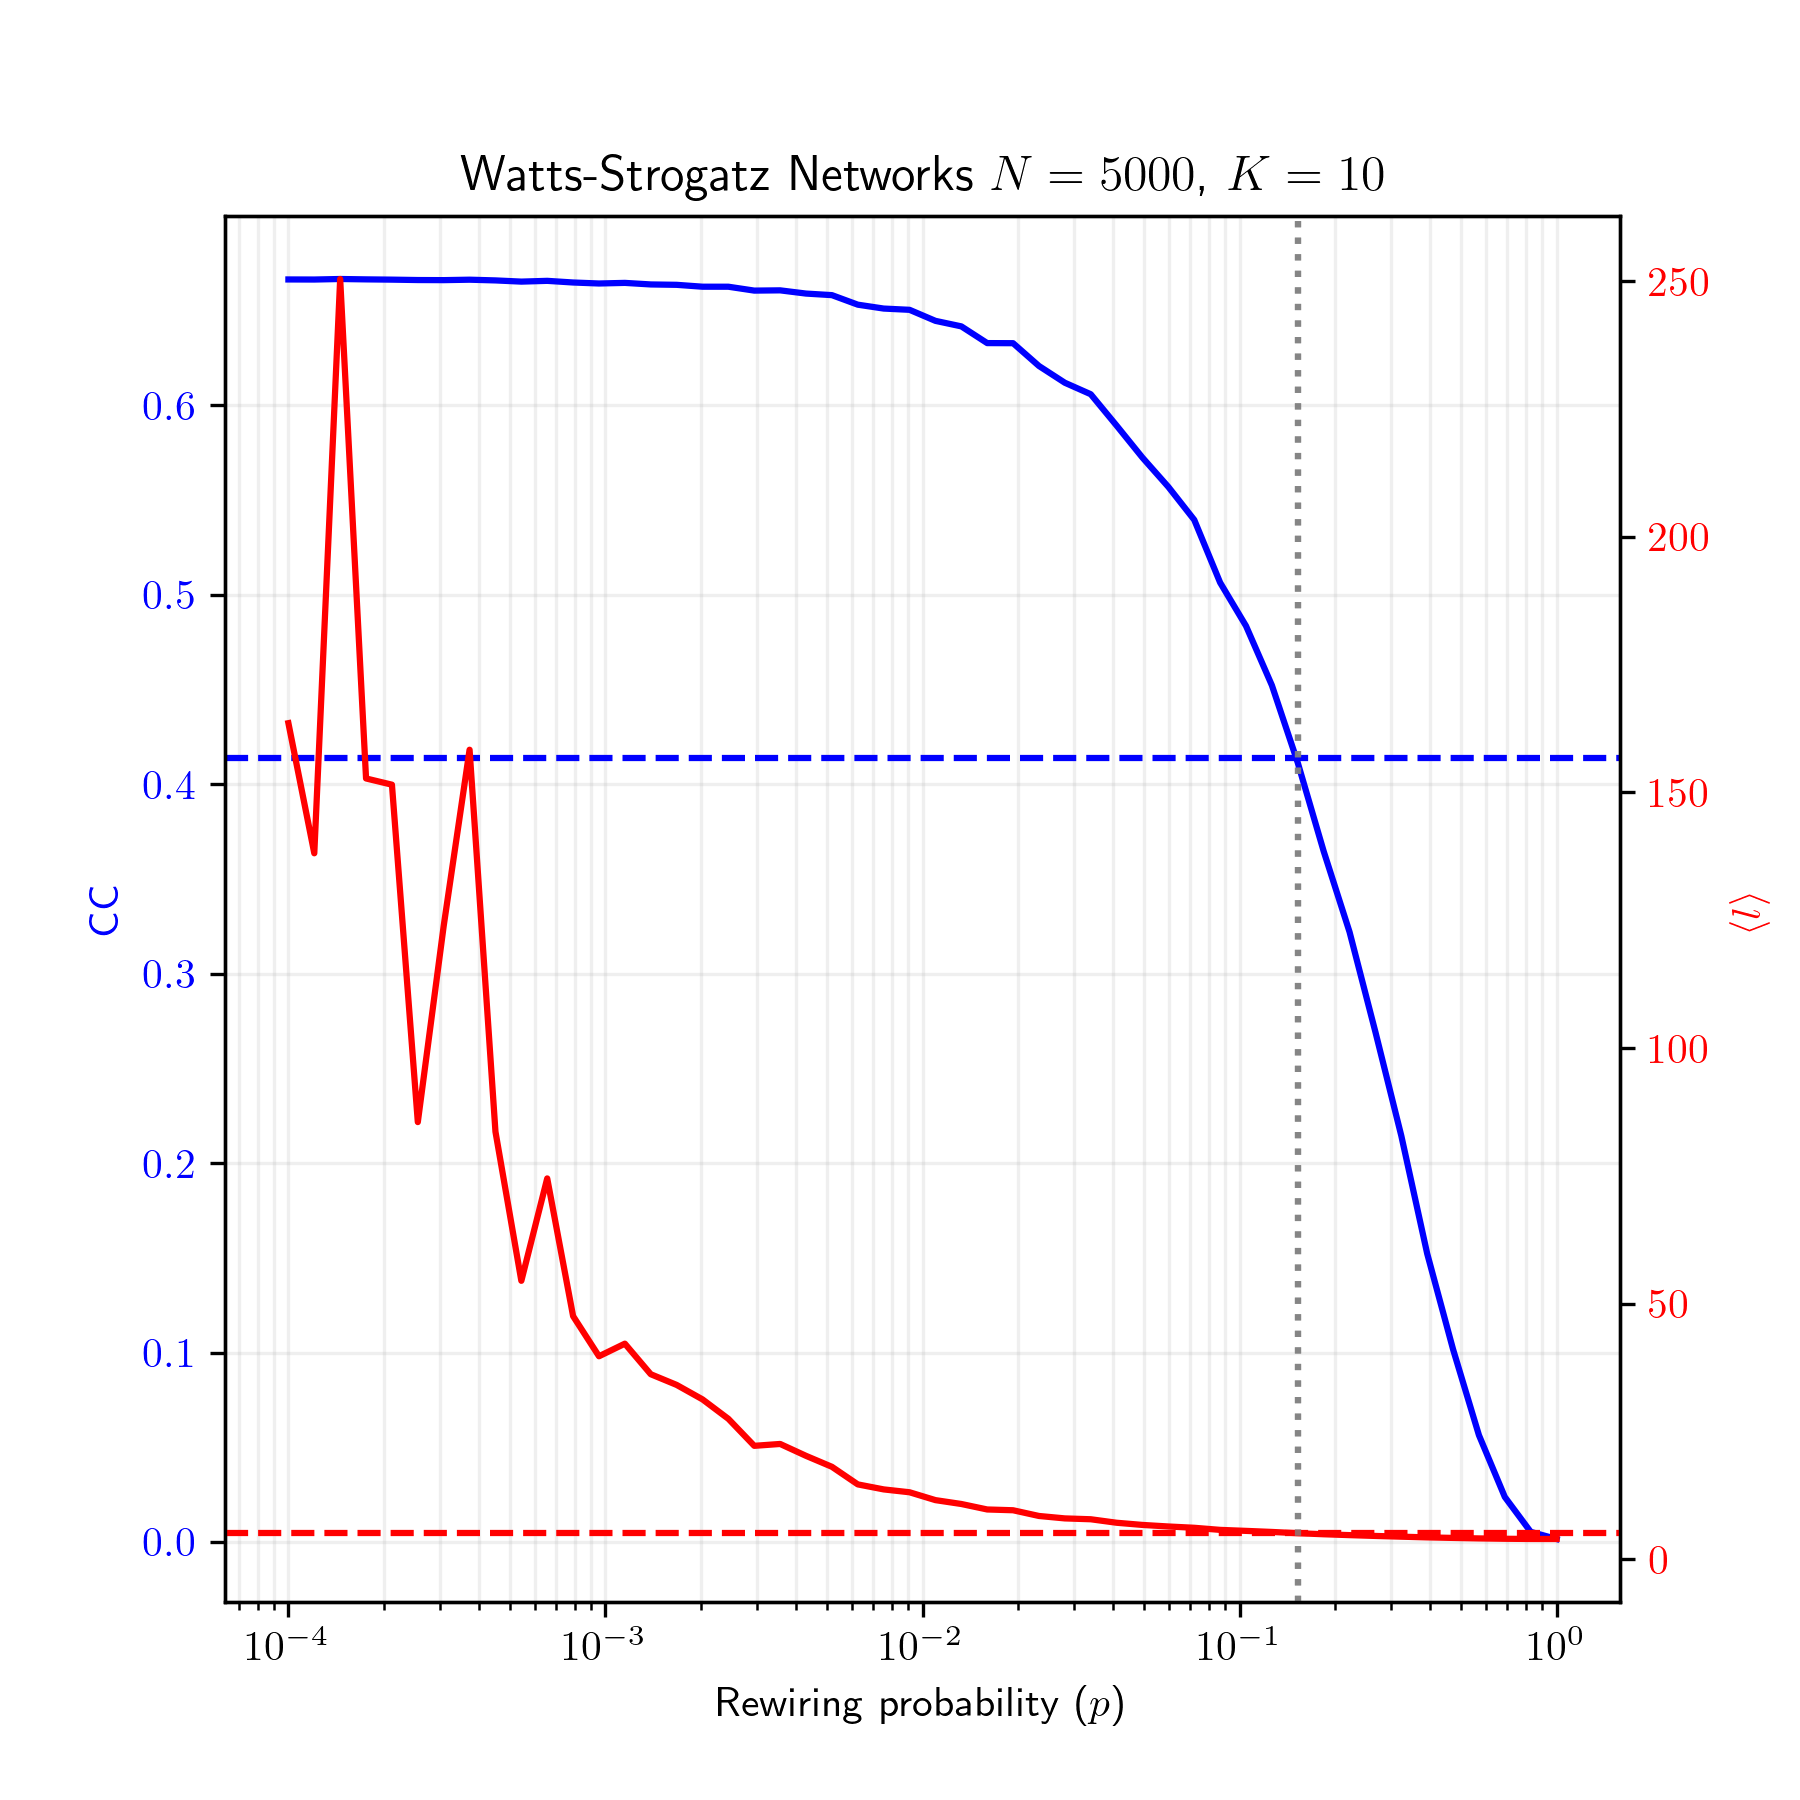
\includegraphics[width=\linewidth]{assets/ws_clustering_aspl.png}
        \caption{Average $\text{CC}$ and $\langle l \rangle$ of WS networks with $N=5000$ and $K=10$ for different values of the rewiring probability $p$. The horizontal dashed lines represent the true values of $\text{CC}$ and $\langle l \rangle$ for the first network. The vertical dashed line represents the value of $p$ that best matches these values ($p = 0.1526$).}
        \label{fig:ws_clustering_path_length}
    \end{minipage}\hfill
    \begin{minipage}{0.55\textwidth}
        \centering
        \small
        \begin{tabular}{lcc}
        \toprule
        \textbf{Metric} & \textbf{$\mu$} & \textbf{$\sigma$} \\
        \midrule
        Number of nodes & 5000 & 0.0 \\
        Number of edges & 25000 & 0.0 \\
        Max degree & 15.26 & 0.5936 \\
        Min degree & 5.86 & 0.3470 \\
        Average degree & 10 & 0.0 \\
        Avg. clustering coefficient & 0.4144 & 0.0033 \\
        Degree assortativity & -0.0124 & 0.0054 \\
        Avg. shortest path length & 5.1209 & 0.0167 \\
        Diameter & 8 & 0.0 \\
        \bottomrule
        \end{tabular}
        \captionof{table}{Mean and standard deviation of the metrics of 50 different random networks generated with the WS model with parameters $N=5000$, $K=10$ and $p=0.15$.}
        \label{tab:ws_metrics}
    \end{minipage}
\end{figure}


\begin{enumerate}
    \setcounter{enumi}{1}
    \item Theoretically. The average clustering coefficient of a WS network can be approximated by $\text{CC}(p) = \text{CC}(0)(1-p)^3$, where $\text{CC}(0) = \frac{3(K-2)}{4(K-1)}$ is the clustering coefficient of the original lattice (equation 2.22 in \cite{boccaletti2006complex}). Setting the known values for $\text{CC}(p)$ and $\text{CC}(0)$, and solving for $p$ gives:
    \begin{equation}
        p = 1 - \left(\frac{\text{CC}(p)}{\text{CC}(0)}\right)^{\frac{1}{3}} = 1 - \left(\frac{0.4141}{0.375}\right)^{\frac{1}{3}} \approx 0.147
    \end{equation}
\end{enumerate}

In both cases, the estimated value of $p$ is around 0.15. Therefore, the parameters of the WS model that generates the first network are $N=5000$, $K=10$ and $p=0.15$. To further support this conclusion, the same metrics reported in \Cref{tab:network_characterization} were computed for 50 different random networks generated with these parameters. The mean and the standard devation these metrics are reported in \Cref{tab:ws_metrics}. Note that the mean values of these metrics are very close to the values of the first network, and the standard deviation is relatively low.


\subsection{Network 2: Erdös-Rényi Model}  % ER 0.0021 maria

The second network is generated by the ER model~\cite{erdds1959random}. One of the most used formulations of this model is the one proposed by Gilbert~\cite{gilbert1959random}, where a graph is generated by connecting nodes randomly. Each edge is included in the graph with a probability $p$ independent from every other edge. The resulting graph is denoted as $G(N, p)$, where $N$ is the number of nodes and $p$ is the probability of edge creation.

There are several properties of the second network that suggest that it has been generated by an ER model. In an ER model, the degree distribution follows a binomial distribution, which can be approximated by a Poisson distribution for large $N$ and small $p$ as
\begin{equation}
    P(k) \approx \frac{e^{-\langle k \rangle} \langle k \rangle^k}{k!}.
\end{equation}
This results in a homogeneous degree distribution where most nodes have degrees close to the average degree $\langle k \rangle$. As shown in Figure~\ref{fig:net2_hist}, the degree distribution of the second network is indeed homogeneous, with a maximum degree of 24 and an average degree of around 10. Figure~\ref{fig:net2_poisson} shows the degree distribution of the second network along with the Poisson distribution with the same average degree. The degree distribution of the second network closely follows the Poisson distribution, which is a strong indication that it has been generated by an ER model.

Moreover, the ER network does not capture the high clustering coefficient that is present in many real networks, and \textit{net2} has a very low average clustering coefficient of 0.0021. Finally, the ER model captures the small-world property, which is also present in the second network, as it has a small average shortest path length (3.9560) and a small diameter (7) relative to its size (5000 nodes).

The parameter $p$ of the ER model can be estimated using the clustering coefficient of the \textit{net2}. In an ER model, $\text{CC} = p$. Therefore, the estimated value of $p$ is 0.0021. Therefore, the parameters of the ER model that generates the second network are $N=5000$ and $p=0.0021$. To further support this conclusion, the same metrics reported in \Cref{tab:network_characterization} were computed for 50 different random networks generated with these parameters. It is important to realize that the resulting networks are not guaranteed to be connected. Therefore, only the largest connected component of each generated network was considered for the calculation of the metrics. As a result, some networks do not have exactly 5000 nodes. Table~\ref{tab:er_metrics} shows the mean and standard deviation of the metrics of these 50 different random networks. The mean values of these metrics are very close to the values of the second network, and the standard deviation is relatively low. The only exception is the number of edges, which is higher than the one of the second network. This is because the number of edges in an ER network follows a binomial distribution with parameters $n = \binom{N}{2}$ and $p$, so they are not fixed. This higher number of edges also has an impact on the slightly higher average degree and maximum degree of the generated networks compared to the second network.

\begin{figure}[htbpt]
    \centering
    \begin{minipage}{0.4\textwidth}
        \centering
        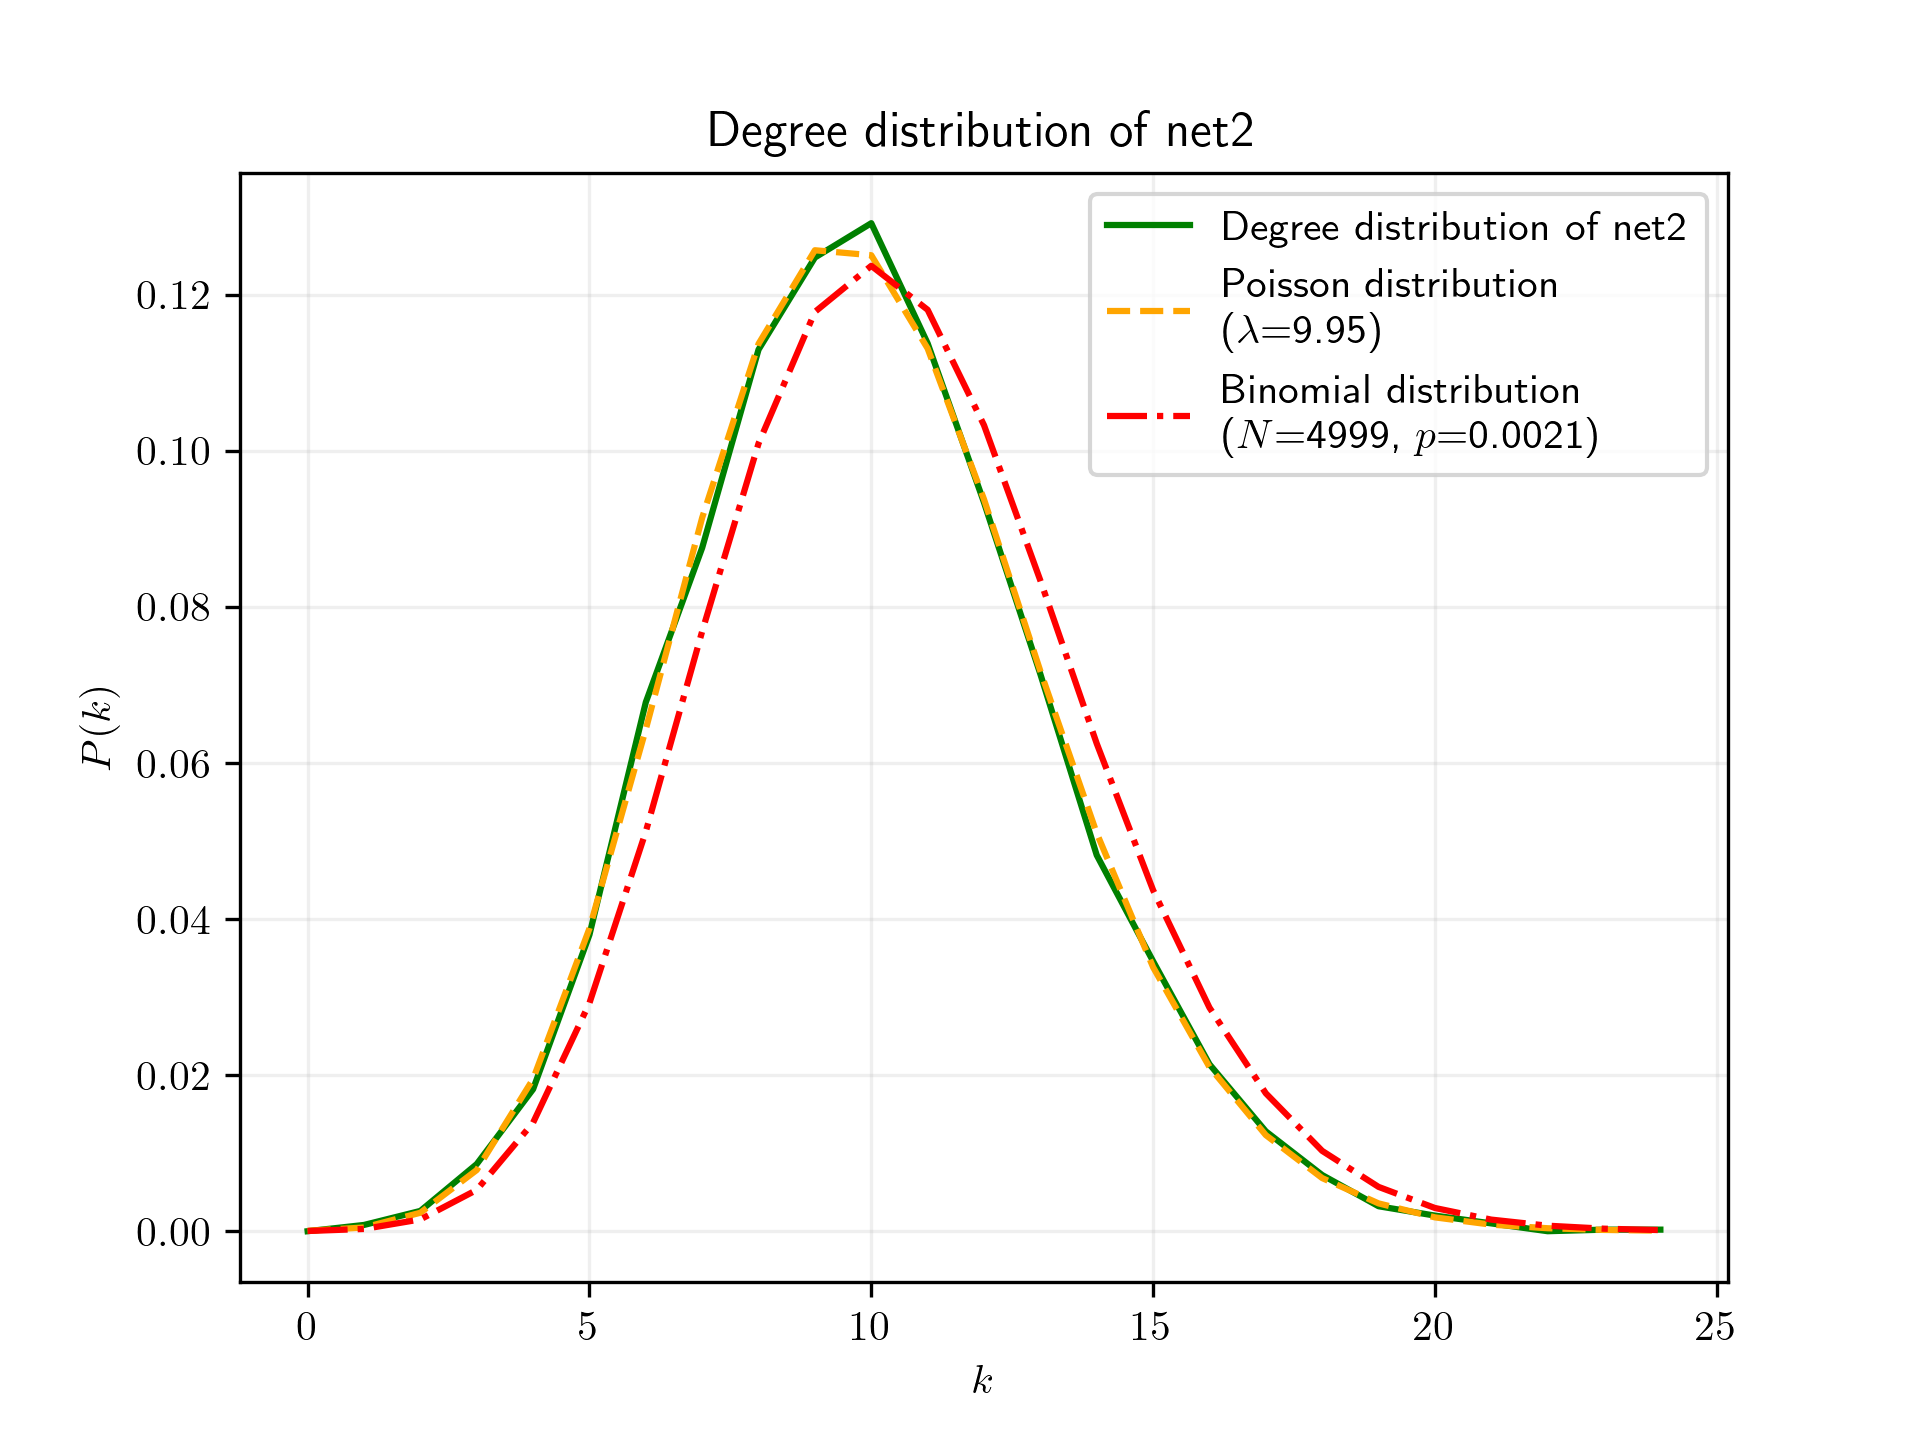
\includegraphics[width=\linewidth]{assets/net2_degree_poisson_binomial.png}
        \caption{Degree distribution of the second network (green) along with the Poisson distribution (orange) with the same average degree and a binomial distribution (red) with parameters $n = N-1$ and $p$.}
        \label{fig:net2_poisson}
    \end{minipage}\hfill
    \begin{minipage}{0.55\textwidth}
        \centering
        \small
        \begin{tabular}{lcc}
            \toprule
            \textbf{Metric} & \textbf{$\mu$} & \textbf{$\sigma$} \\
            \midrule
            Number of nodes & 4999.8400 & 0.3666 \\
            Number of edges & 26258.5200 & 168.7282 \\
            Max degree & 24.4400 & 1.4023 \\
            Min degree & 1.2400 & 0.4271 \\
            Average degree & 10.5037 & 0.0675 \\
            Avg. clustering coefficient & 0.0021 & 0.0002 \\
            Degree assortativity & -0.0002 & 0.0063 \\
            Avg. shortest path length & 3.8733 & 0.0093 \\
            Diameter & 6.3200 & 0.4665 \\
            \bottomrule
            \end{tabular}
            \captionof{table}{Mean and standard deviation of the metrics of 50 different random networks generated with the ER model with parameters $N=5000$ and $p=0.0021$.}
            \label{tab:er_metrics}
    \end{minipage}
\end{figure}


\subsection{Network 3: Configuration Model}\label{sec:cm} % CM gamma = 2.5 A

The third network is generated by the Configuration Model (CM)~\cite{bollobas1980probabilistic}. The CM is a random graph model that generates a random network subject to a certain degree sequence. Given a target sequence of degrees $\{k_1, k_2, \ldots, k_N\}$, each node $i$ is assigned $k_i$ stubs (half-edges), and the stubs are then randomly paired uniformly at random to form edges. The resulting graph may include self-loops and multiple edges, but it preserves the degree sequence exactly.

A key advantage of the CM over other models is that the degree distribution can be chosen freely. In particular, it can follow a power-law $P(k)\sim k^{-\gamma}$ with any exponent $\gamma$, including values $\gamma < 3$. This flexibility is significant because many real-world networks exhibit power-law degree distributions with exponents in the range $2 < \gamma < 3$. As it will be explained in \Cref{sec:ba}, other models are constrained to $\gamma = 3$, so a CM with $\gamma < 3$ can capture a wider class of scale-free topologies.

Several structural properties of \textit{net3} are consistent with a CM origin. Both the $\langle l \rangle = 3.0082$  and the diameter $D = 5$ are very small relative to the number of nodes $N = 5000$, consistent with the scale-free nature of the network (as it has been shown in the degree distribution in previous section). The strongest evidence comes from the degree distribution. Figure~\ref{subfig:net3_ccdf} shows the CCDF of the degree distribution of the third network in log-log space. Fitting a line to the CCDF in log-log space gives an estimated value of $\gamma = 2.3363$ (see \Cref{fig:cm_degree_distribution}), which is consistent with a model that can generate power-law degree distributions with variable $\gamma$ values, such as the CM.

\begin{figure}[htbpt]
    \centering
    \begin{minipage}{0.4\textwidth}
    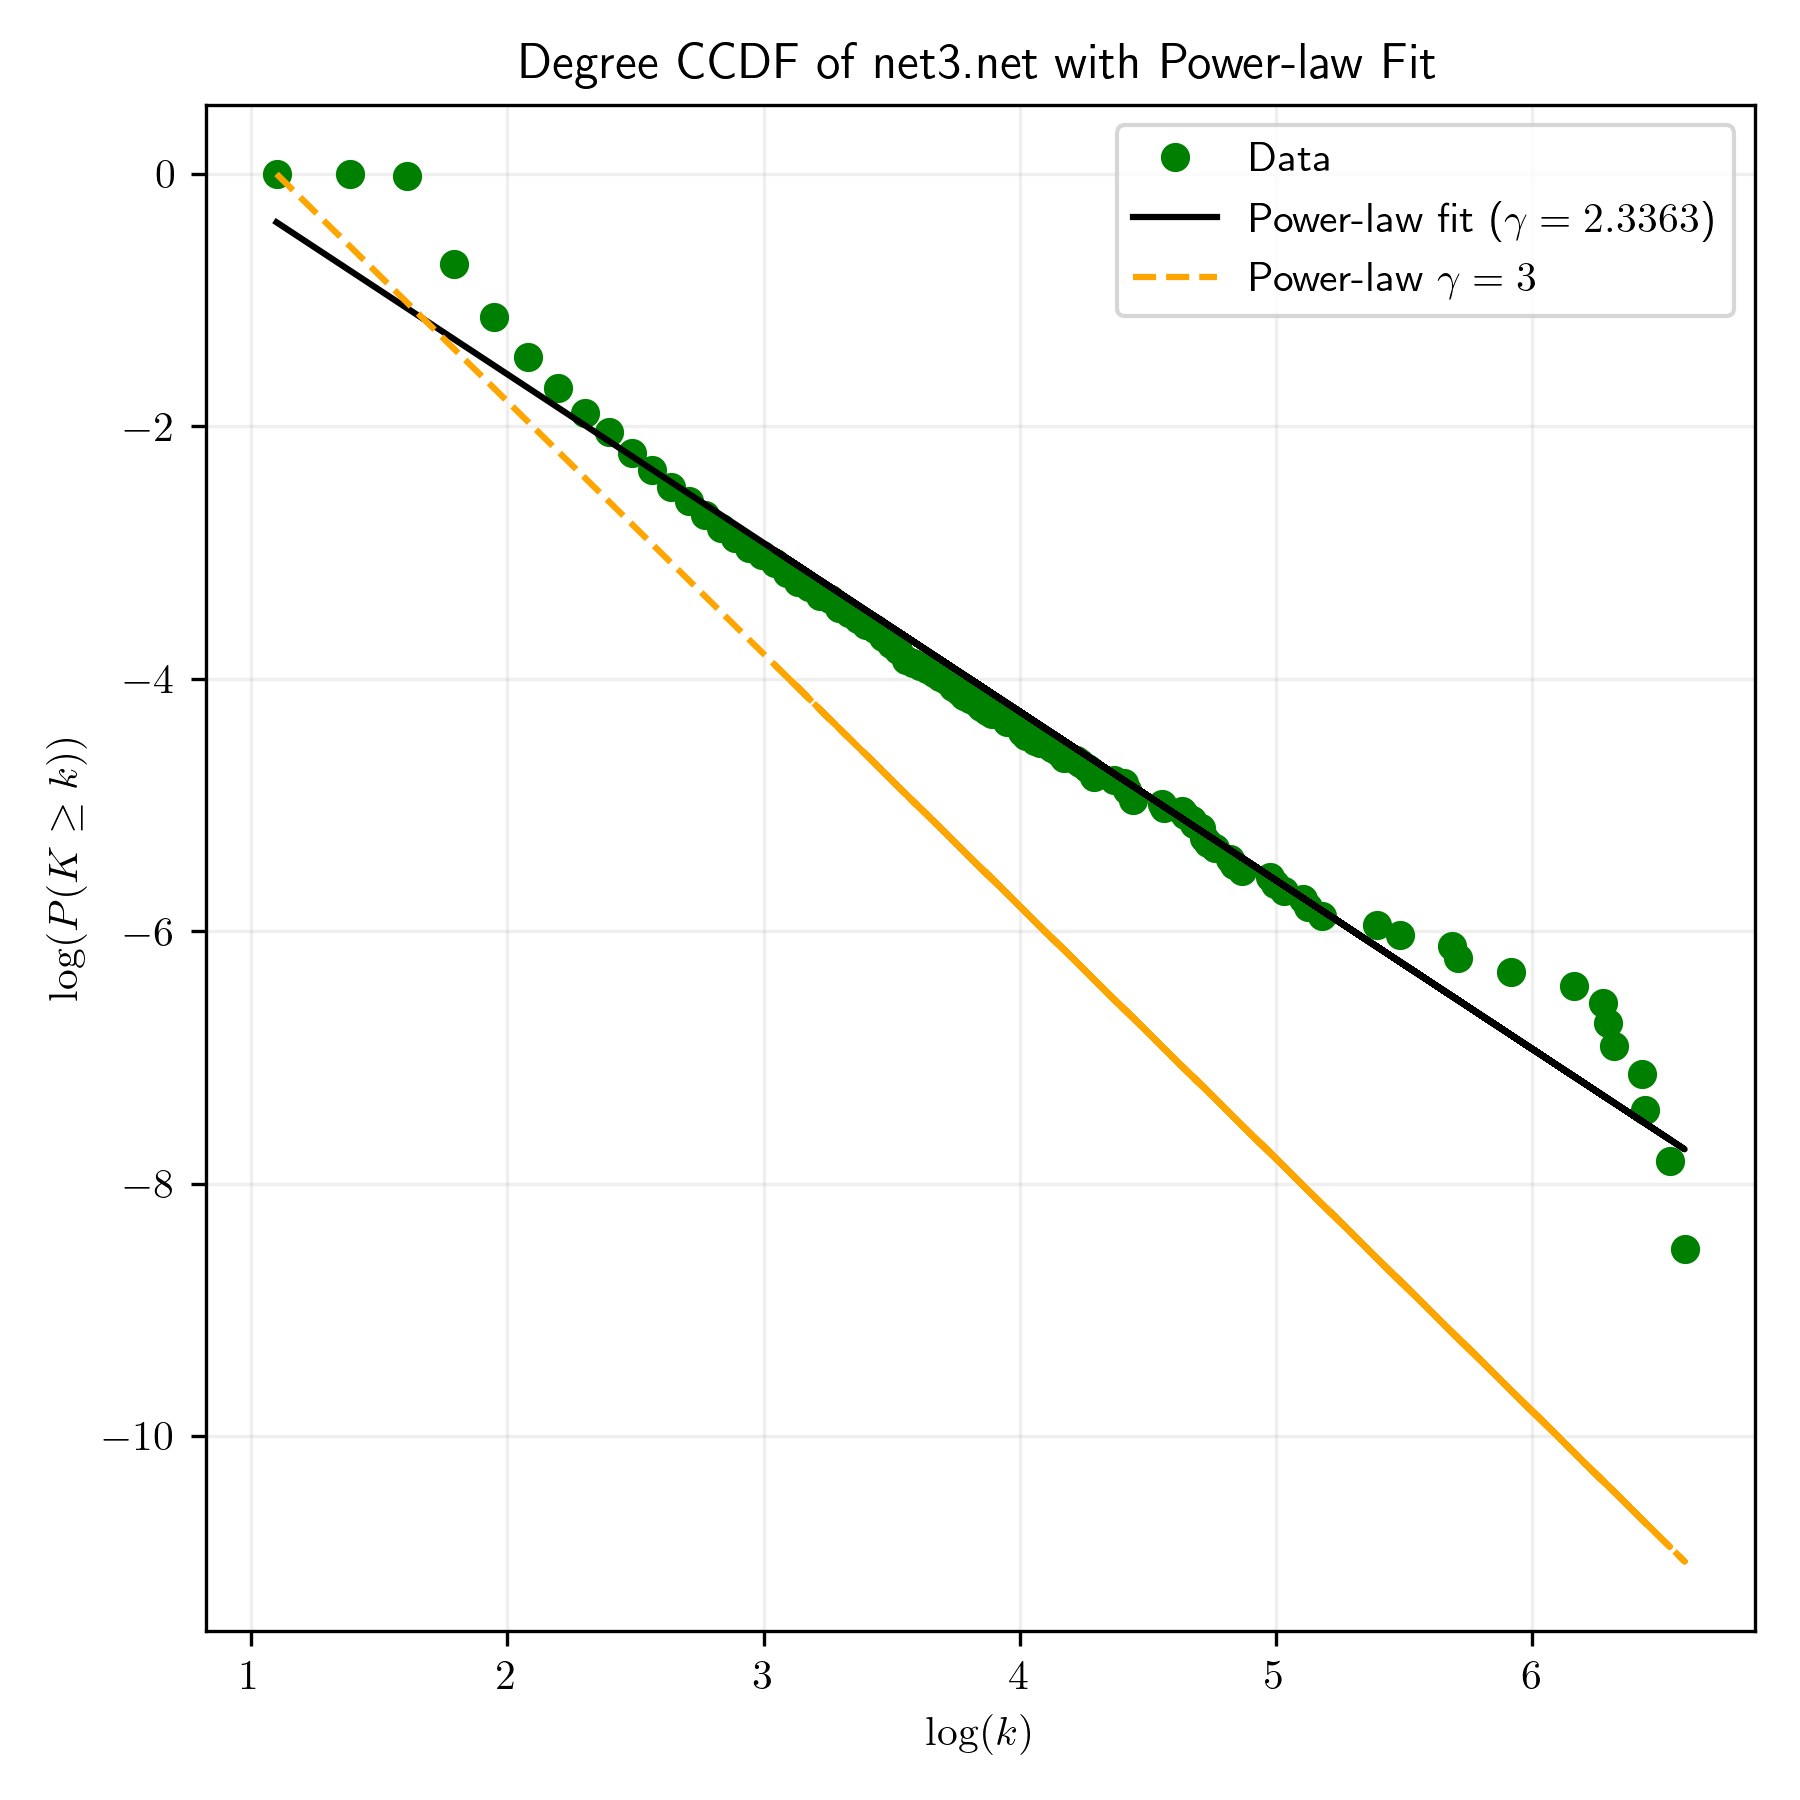
\includegraphics[width=\textwidth]{assets/cm_ccdf_fit.png}
    \caption{CCDF of the degree distribution of the third network in log-log space. The black line shows the power law fit. The estimated value of the exponent $\gamma$ is 2.3363, which is consistent with a model that can generate power-law degree distributions with variable $\gamma$ values, such as the CM. The dashed orange line represents a power law with $\gamma = 3$.}
    \label{fig:cm_degree_distribution}
    \end{minipage}\hfill
    \begin{minipage}{0.55\textwidth}
        \centering
        \small
        \begin{tabular}{lcc}
        \toprule
        \textbf{Metric} & \textbf{$\mu$} & \textbf{$\sigma$} \\
        \midrule
        Number of nodes & 5000 & 0.0 \\
        Number of edges & 22615.62 & 21.8677 \\
        Max degree & 573.96 & 10.0458 \\
        Min degree & 3.0 & 0.0 \\
        Average degree & 9.0462 & 0.0087 \\
        Avg. clustering coefficient & 0.0587 & 0.0011 \\
        Degree assortativity & -0.1024 & 0.0012 \\
        Avg. shortest path length & 3.1383 & 0.0048 \\
        Diameter & 5.42 & 0.4936 \\
        \bottomrule
        \end{tabular}
        \captionof{table}{Mean and standard deviation of the metrics of 50 different random networks generated with the CM from the degree sequence of the third network.}
        \label{tab:cm_metrics}
    \end{minipage}
\end{figure}

\Cref{tab:cm_metrics} shows the mean and standard deviation of the metrics of 50 different random networks generated with the CM from the degree sequence of the third network. To be able to calculate all the metrics, parallel edges and self-loops of the generated networks were removed. In general, all the metrics except the number of edges and the maximum degree are very close to the values of the third network, and the standard deviation is relatively low. The number of edges is slightly lower than the one of the third network because of the removal of parallel edges and self-loops. It is for this same reason that the maximum degree is significantly lower than the one of the third network, as the node with the highest degree is more likely to form self-loops and multiple connections to the same neighbor. These claims are further supported by the results depicted in \Cref{fig:cm_degree_correlation}. It can be seen how the degree of nodes in the third network is highly correlated with the degree of the same nodes in the generated random networks. Overall, the spearman correlation coefficient is 0.9417. However, this correlation is stronger for low-degree nodes than for high-degree nodes, as the latter are more affected by the removal of parallel edges and self-loops.

\begin{figure}[hbtp]
    \centering
    
\includegraphics[width=0.4\textwidth]{assets/cm_degree_correlation.png}
    \caption{Correlation between the degrees of nodes from the third network and the generated random networks.}
    \label{fig:cm_degree_correlation}
\end{figure}




\subsection{Network 4: Barabási-Albert Model}\label{sec:ba} % BA gamma \approx 3 A

The fourth network is generated by the BA model~\cite{barabasi1999emergence}. The BA model is a random graph model that generates scale-free networks through a preferential attachment mechanism. The model generates a network of $N$ nodes by starting with a clique~\footnote{A clique is a graph where every pair of nodes is connected by an edge.} of $m_0$ nodes and then adding the remaining $N - m_0$ nodes one by one. Each new node is connected to $m$ existing nodes with a probability that is proportional to the degree of the existing nodes.

It turns out that the fourth network has a very low average clustering coefficient (0.0107), which is consistent with the BA model, which typically does not generate highly clustered networks. Moreover, the network has a very small $\langle l \rangle$ (3.4868) and diameter (5) compared to the number of nodes $N = 5000$. This indicates the presence of the small-world property, which is also a feature reproduced by the BA model.

However, the strongest evidence comes from the degree distribution. The BA model generates scale-free networks whose degree distribution follows a power law of the form
\begin{equation}
    P(k) \sim k^{-\gamma}
\end{equation}
with exponent $\gamma = 3$. To verify this property, a line in log-log space is fit to the CCDF of the degree distribution. \Cref{fig:ba_degree_distribution} shows the CCDF of the degree distribution of the fourth network in log-log space, along with the fitted line. The estimated value of $\gamma$ is 2.9610, which is close to the expected value of 3 for a BA model. Moreover, the fitted line is very close to the empirical CCDF, which further supports the conclusion that the fourth network is generated by the BA model.

\begin{figure}[htbpt]
    \centering
    \begin{minipage}{0.4\textwidth}
        \centering
        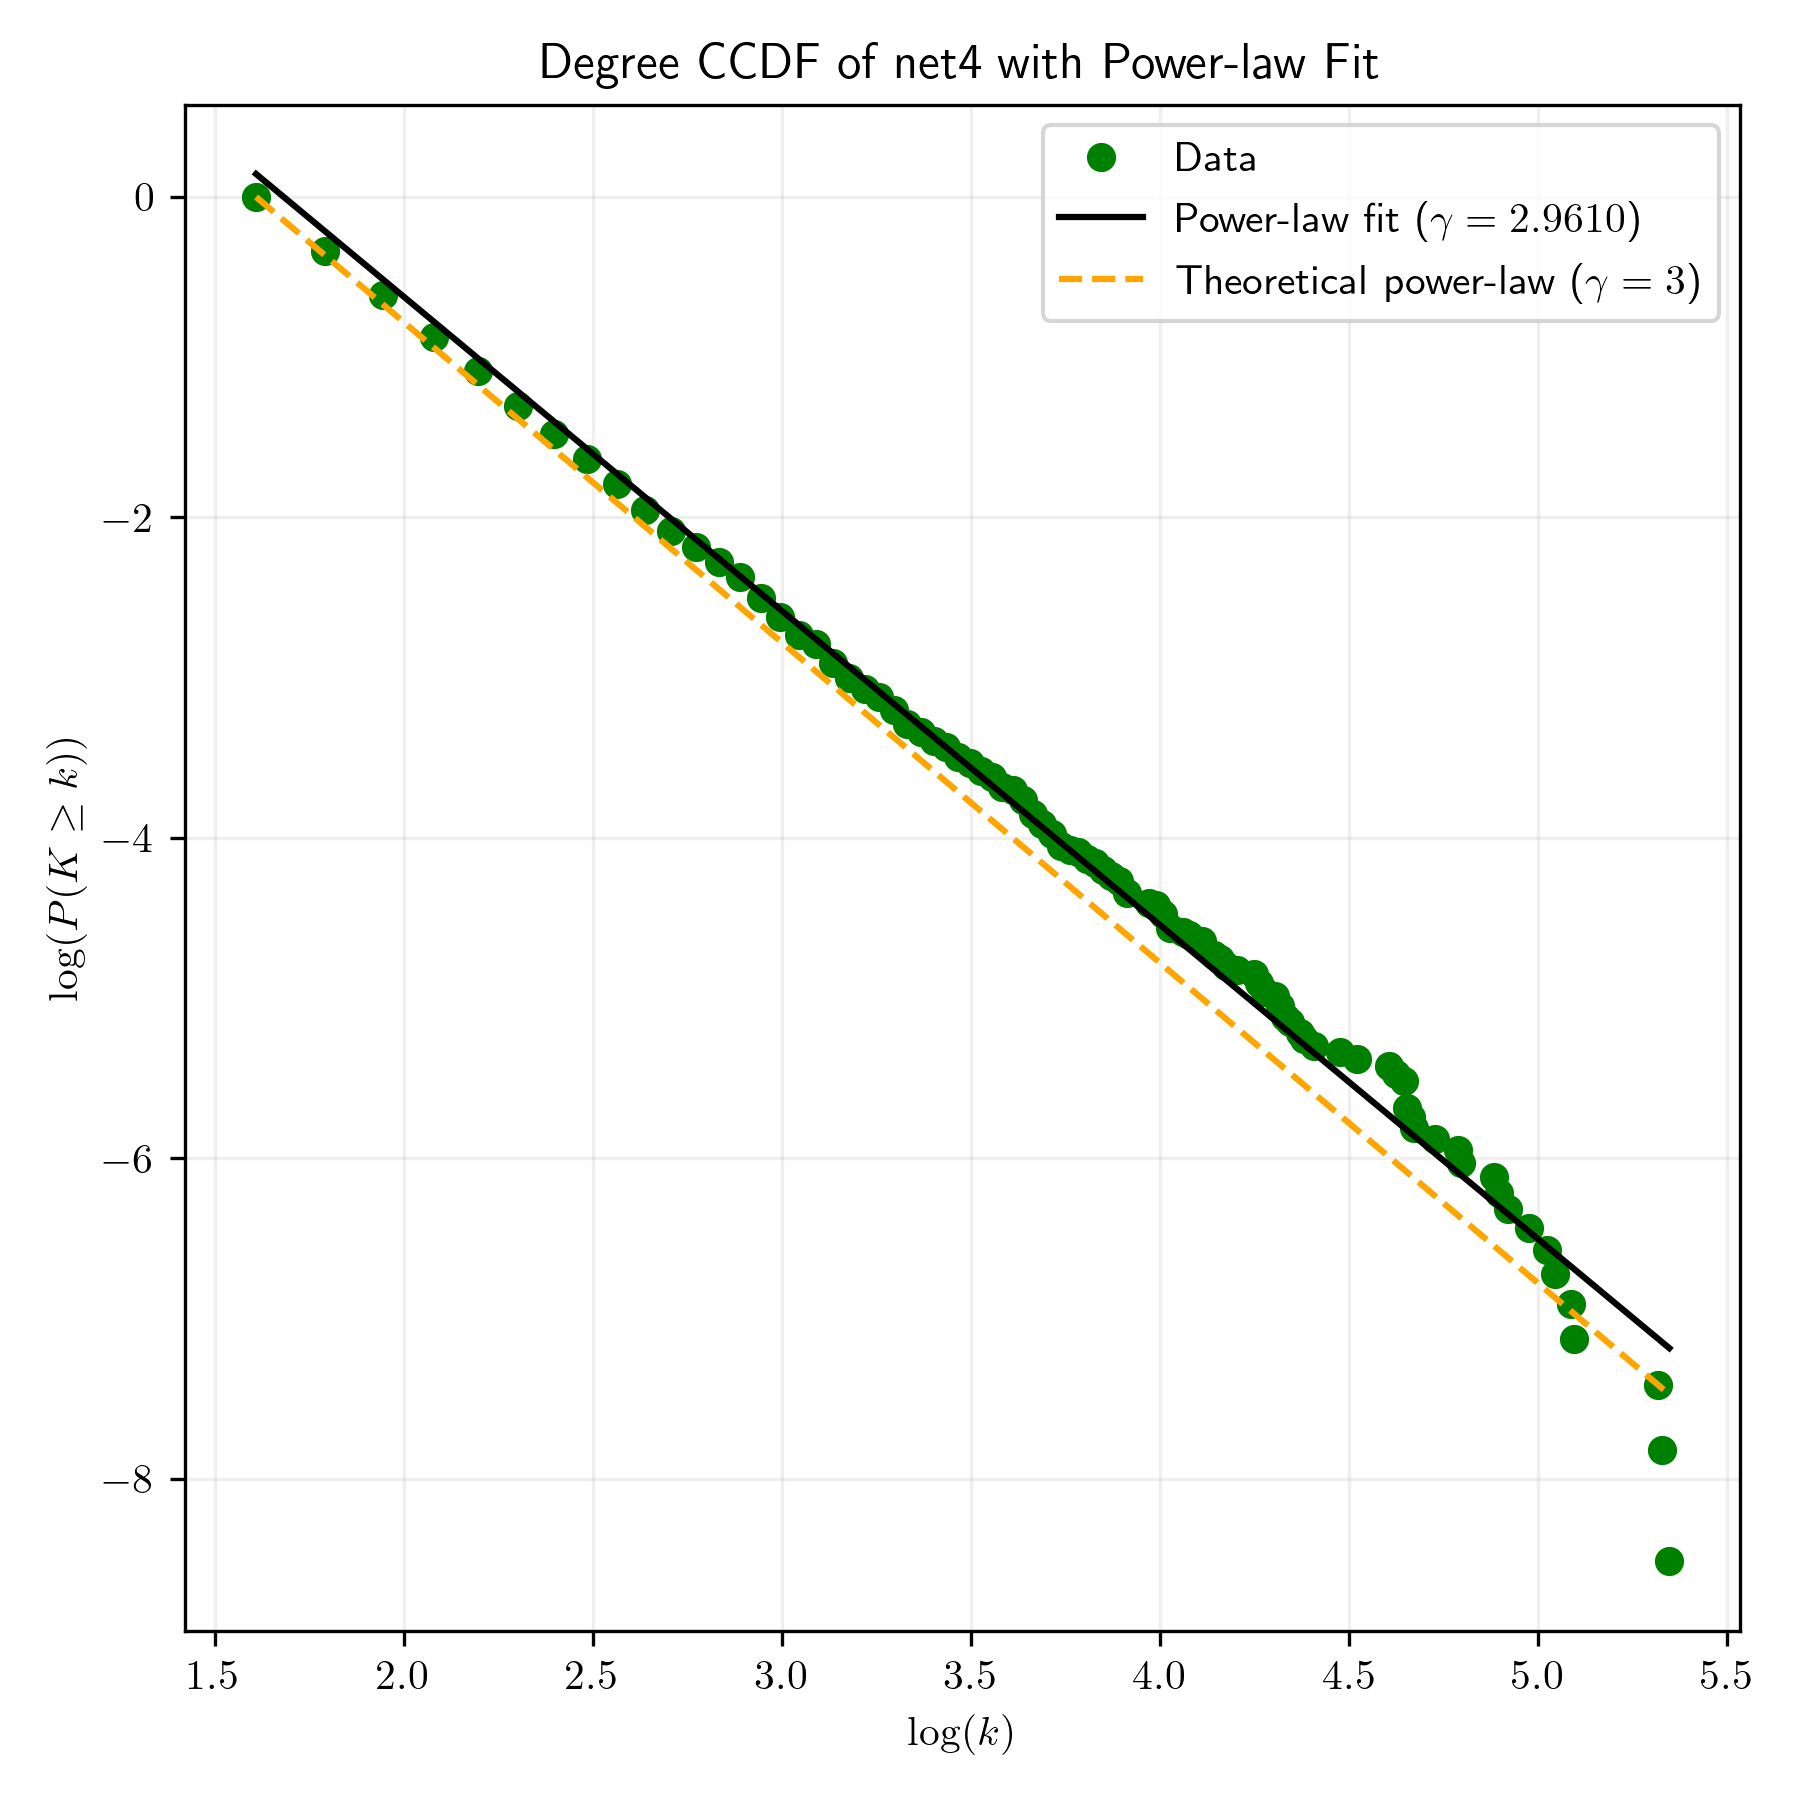
\includegraphics[width=\textwidth]{assets/ba_ccdf_fit.png}
        \caption{CCDF of the degree distribution of the fourth network in log-log space. The black line shows the power law fit. The estimated value of the exponent $\gamma$ is 2.9610, which is close to the expected value of 3 for a BA model, depicted with through the dashed orange line.}
        \label{fig:ba_degree_distribution}
    \end{minipage}\hfill
    \begin{minipage}{0.55\textwidth}
        \centering
        \small
        \begin{tabular}{lcc}
        \toprule
        \textbf{Metric} & \textbf{$\mu$} & \textbf{$\sigma$} \\
        \midrule
        Number of nodes & 5000 & 0.0 \\
        Number of edges & 24975 & 0.0 \\
        Max degree & 275.16 & 39.1818 \\
        Min degree & 5.00 & 0.0 \\
        Average degree & 9.9 & 0.0 \\
        Avg. clustering coefficient & 0.0122 & 0.0008 \\
        Degree assortativity & -0.0355 & 0.0042 \\
        Avg. shortest path length & 3.4634 & 0.0144 \\
        Diameter & 5.1 & 0.3 \\
        \bottomrule
        \end{tabular}
        \captionof{table}{Mean and standard deviation of the metrics of 50 different random networks generated with the BA model with parameters $N=5000$ and $m=5$.}
        \label{tab:ba_metrics}
    \end{minipage}
\end{figure}
The average degree of a network generated by the BA model is $\langle k \rangle = 2m$. Therefore, the parameter $m$ can be estimated as $m = \langle k \rangle / 2 = 9.99 / 2 \approx 5$. Therefore, the parameters that define the BA model that generates the fourth network are $N=5000$ and $m=5$. To further support this conclusion, the same metrics reported in \Cref{tab:network_characterization} were computed for 50 different random networks generated with these parameters. The mean and the standard devation these metrics are reported in \Cref{tab:ba_metrics}. In general, the mean values of these metrics are close to the values of the fourth network and the standard deviation is relatively low, except for the maximum degree, which is highly variable in BA networks. Under the ``\textit{rich-get-richer}'' dynamics, minor differences in the initial connectivity of nodes are amplified over time, leading to significant fluctuations in the maximum degree across different realizations of the network.



\section{Part 3: An extra network} % random geometric graph A


In this section, we analyze the structural properties of an extra network and try to determine the model that generates it. The network contains 200 nodes and 465 edges, which form 7 connected components. The network is depicted in \Cref{fig:extra_network_complete}. All the structural properties that have been calculated in \Cref{sec:part1} cannot be calculated for this network because it is not connected. In these cases, the metrics are calculated for the largest connected component of the network, depicted in \Cref{fig:extra_network_lcc}.

\begin{figure}[hbtp]
    \centering
    \begin{subfigure}[b]{0.45\textwidth}
        \centering
        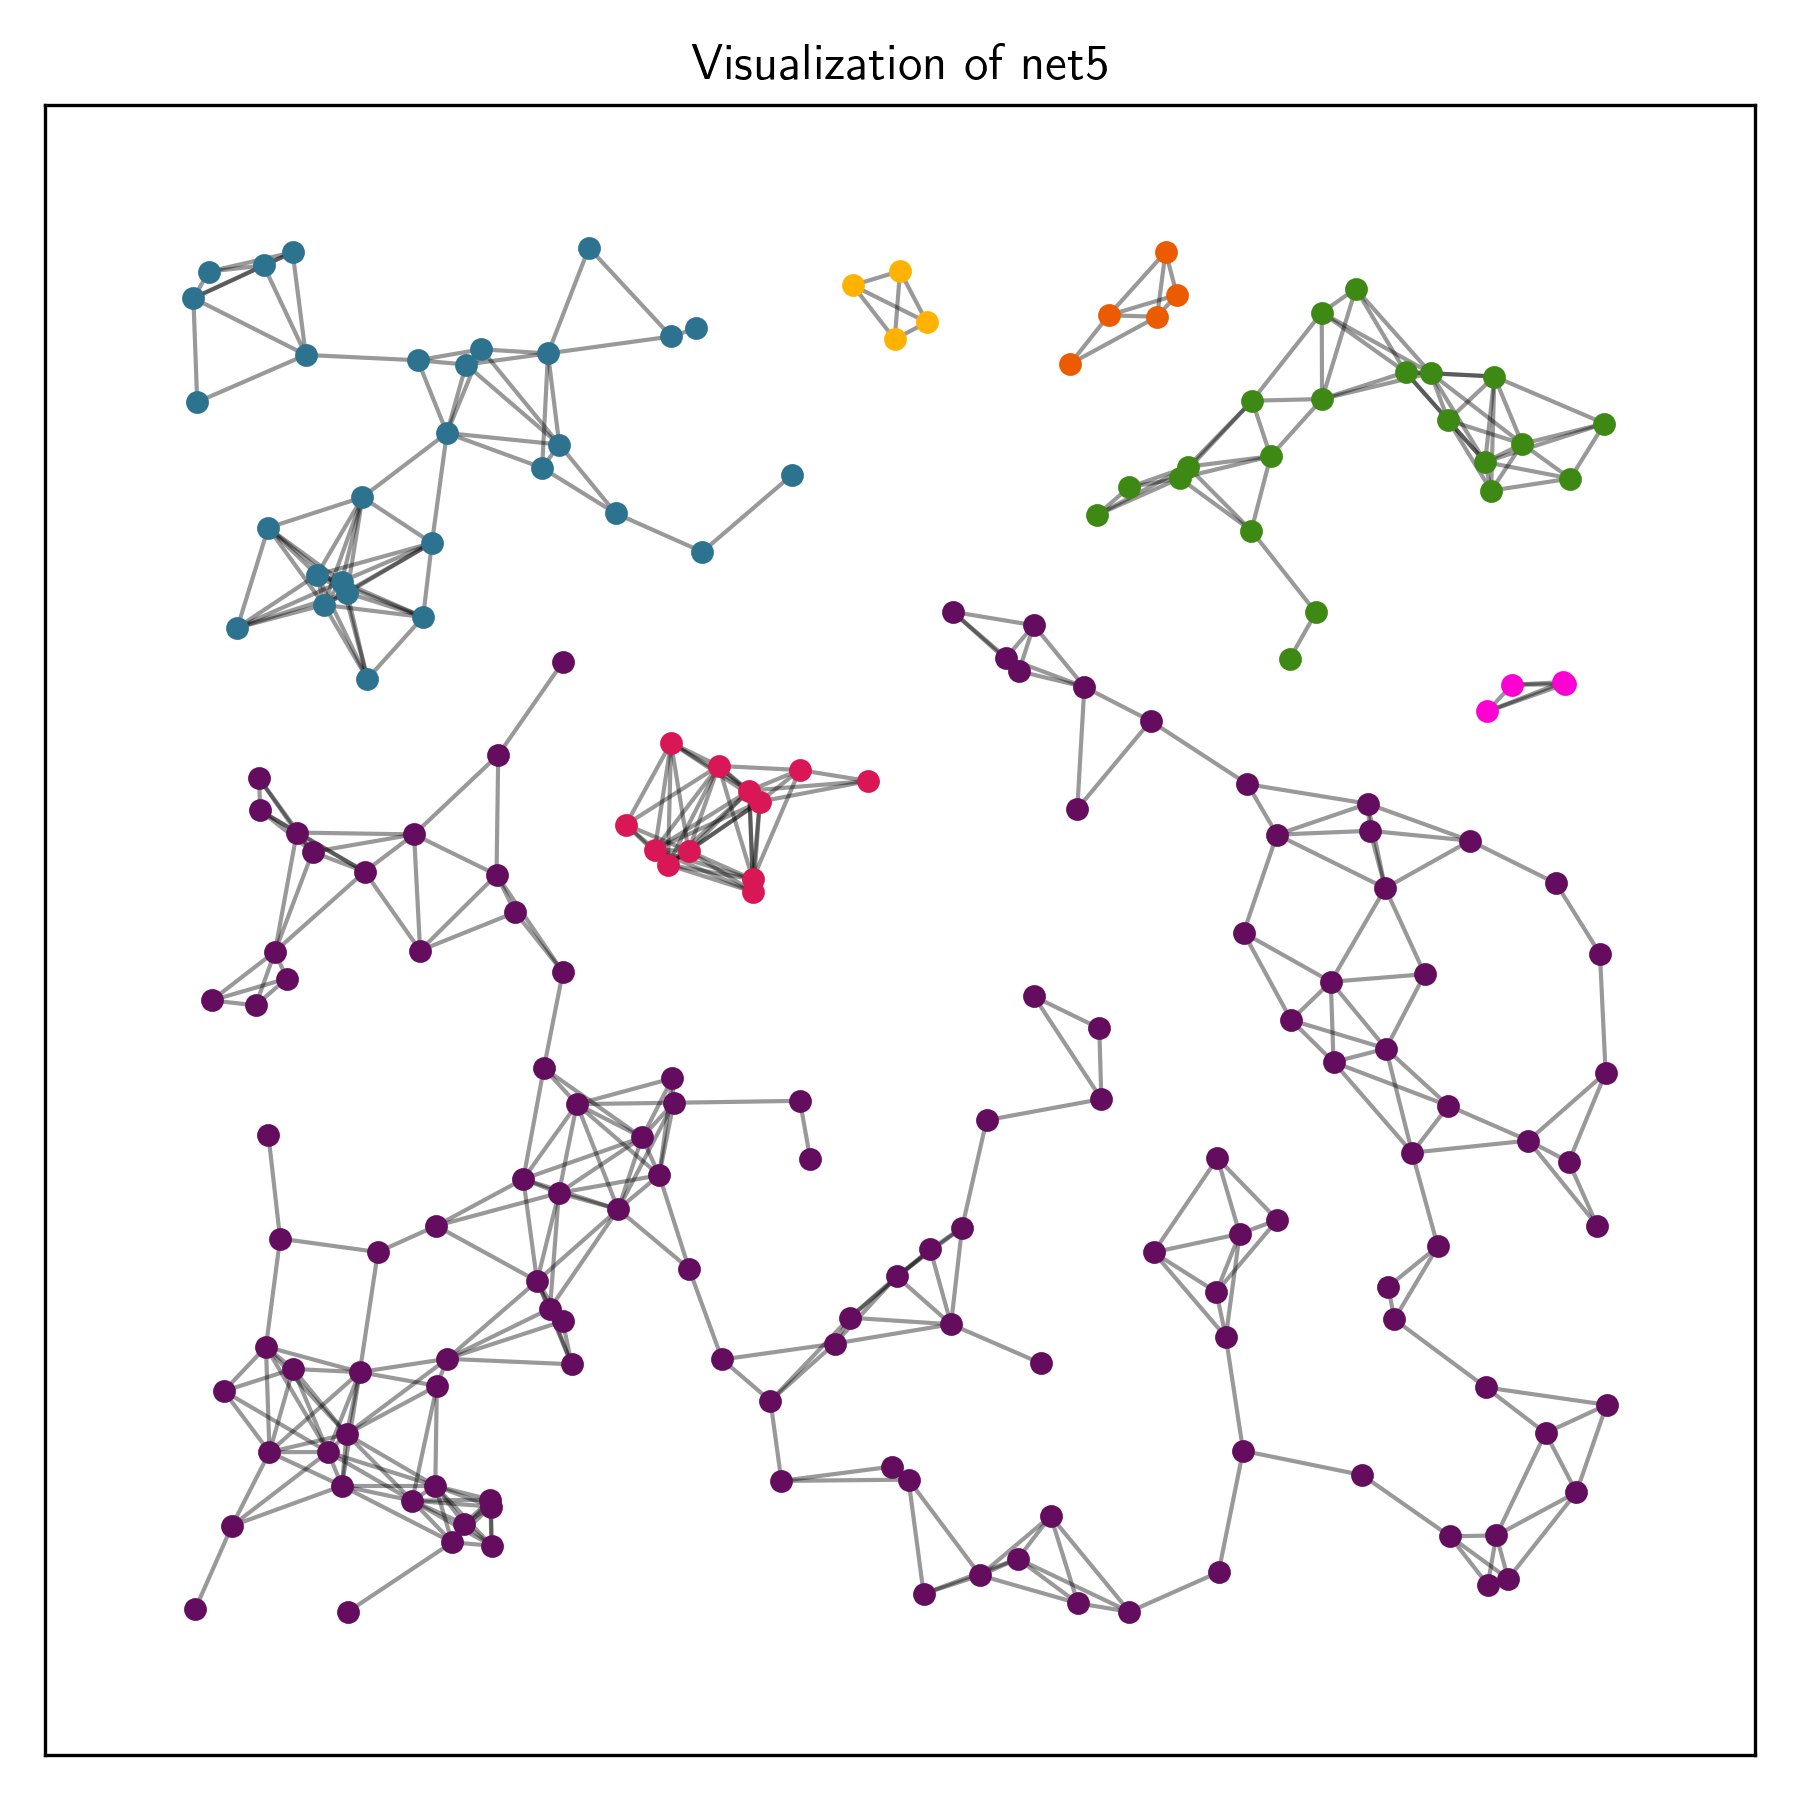
\includegraphics[width=0.8\textwidth]{assets/net5_visualization.png}
        \caption{Complete network.}
        \label{fig:extra_network_complete}
    \end{subfigure}\hfill
    \begin{subfigure}[b]{0.45\textwidth}
        \centering
        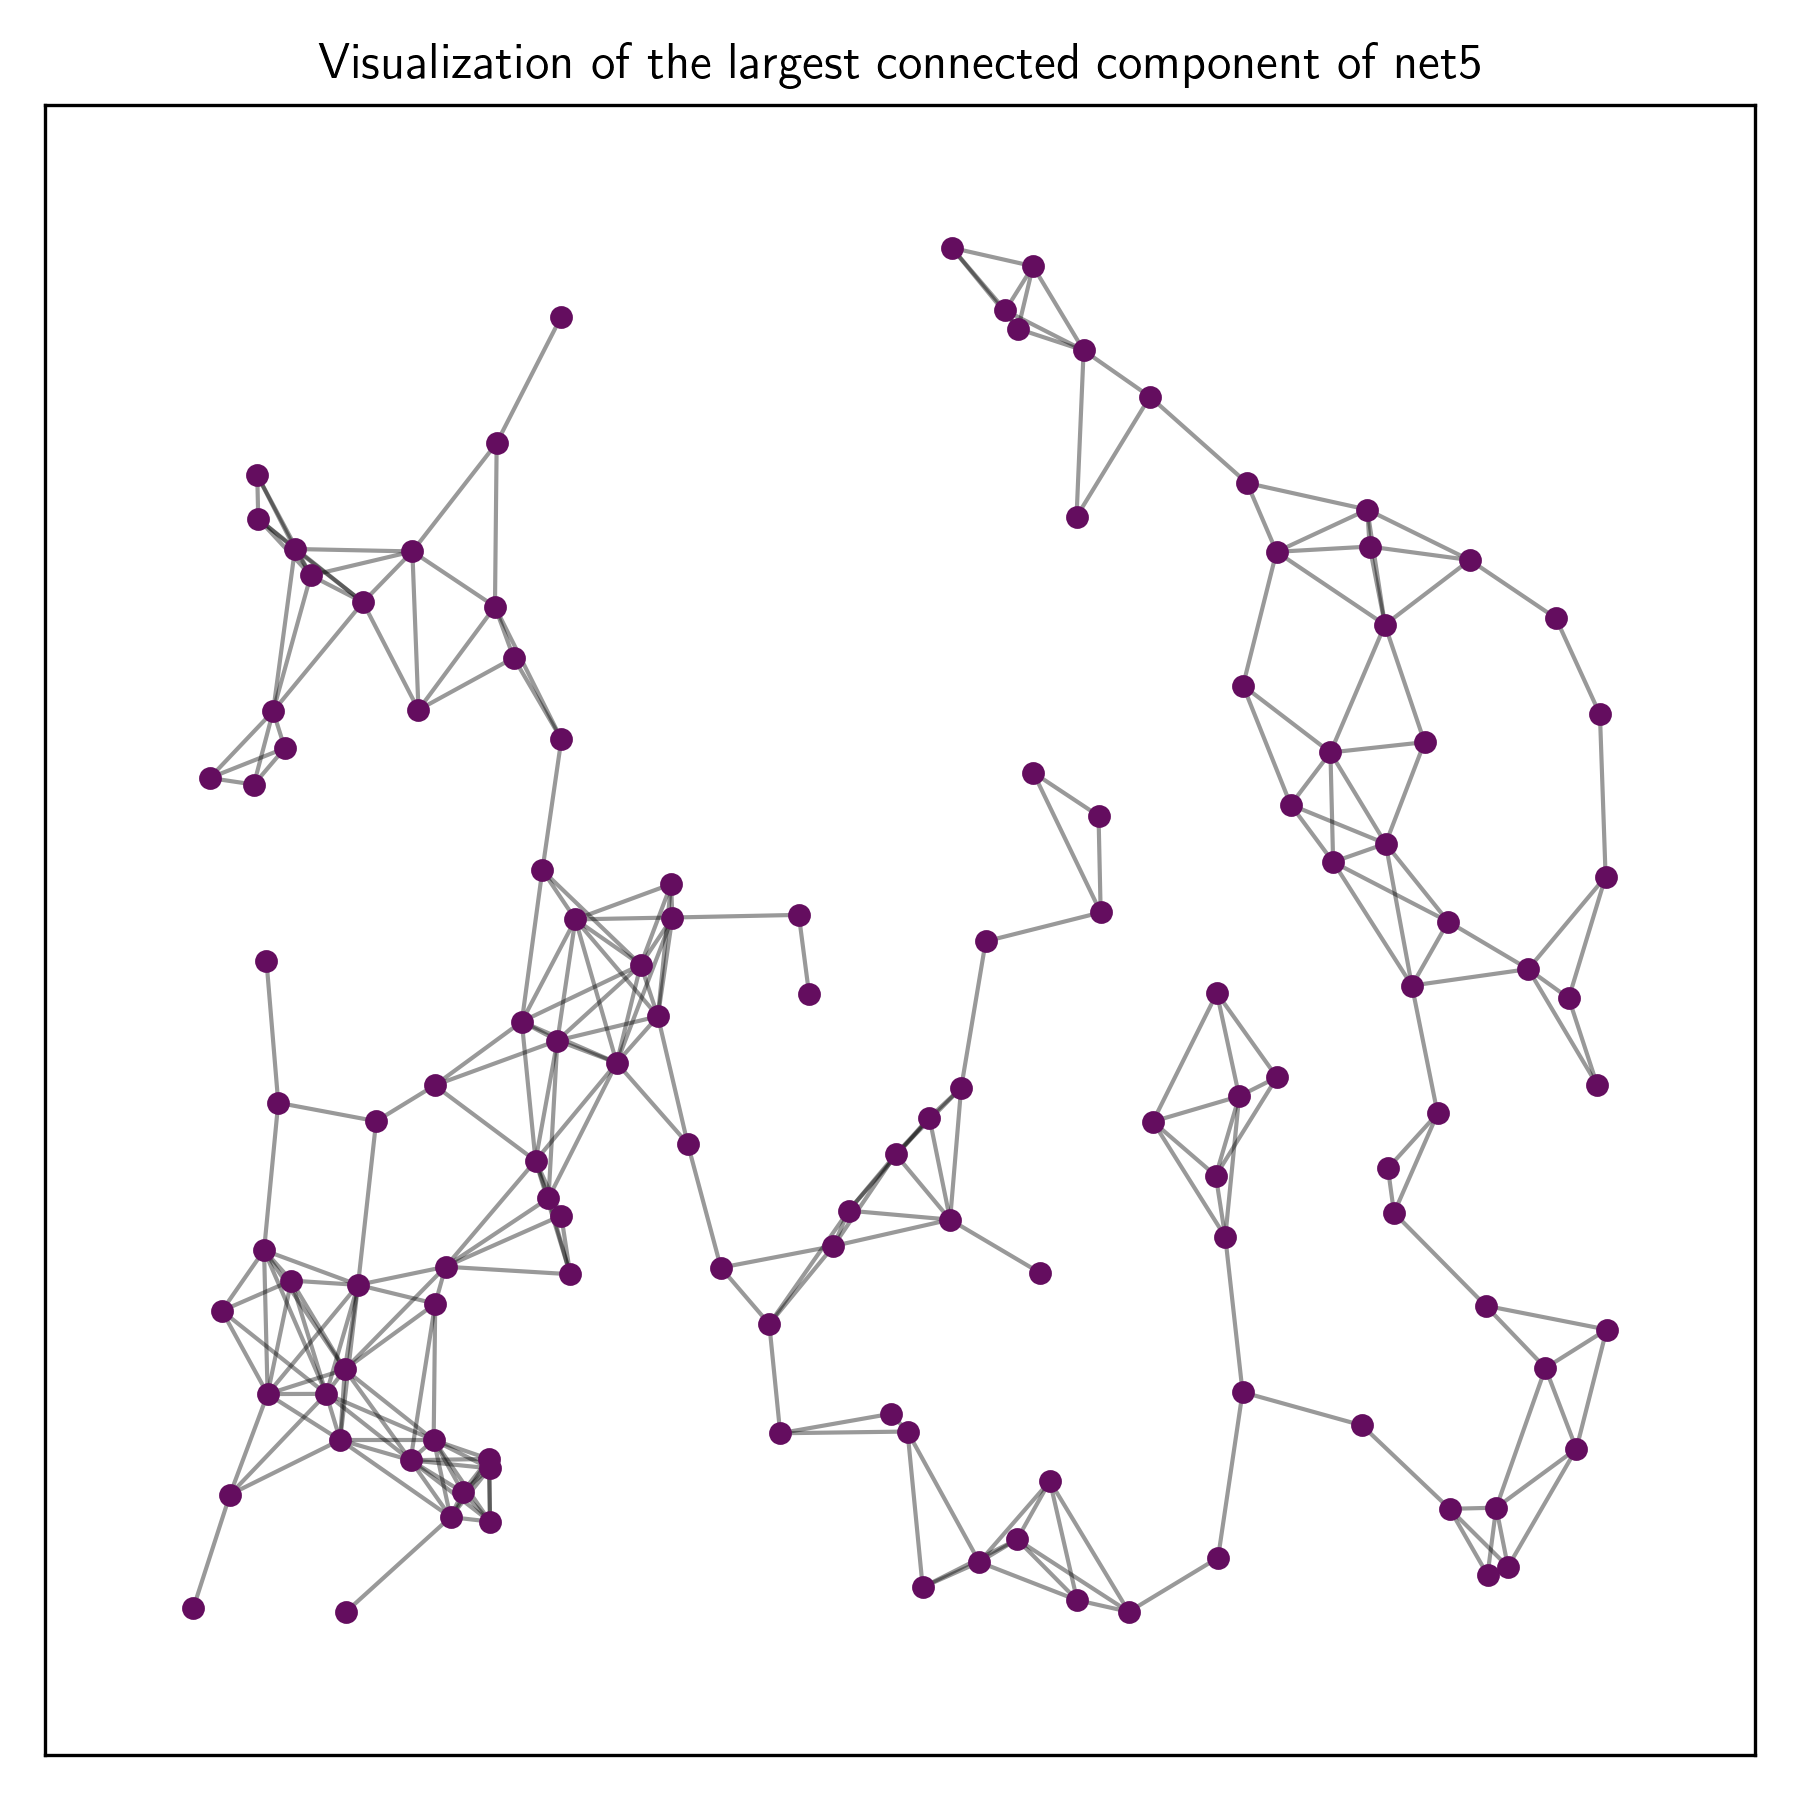
\includegraphics[width=0.8\textwidth]{assets/net5_largest_cc_visualization.png}
        \caption{Largest connected component.}
        \label{fig:extra_network_lcc}
    \end{subfigure}
    \caption{Visualization of the extra network. Left: complete network with all connected components. Right: largest connected component used for structural characterization.}
    \label{fig:extra_network}
\end{figure}


\begin{figure}
    \centering
    \begin{subfigure}[b]{0.45\textwidth}
        \centering
        
\includegraphics[width=0.8\textwidth]{assets/net5_hist.png}
        \caption{Degree distribution of the complete network 5.}
    \end{subfigure}\hfill
    \begin{subfigure}[b]{0.45\textwidth}
        \centering
        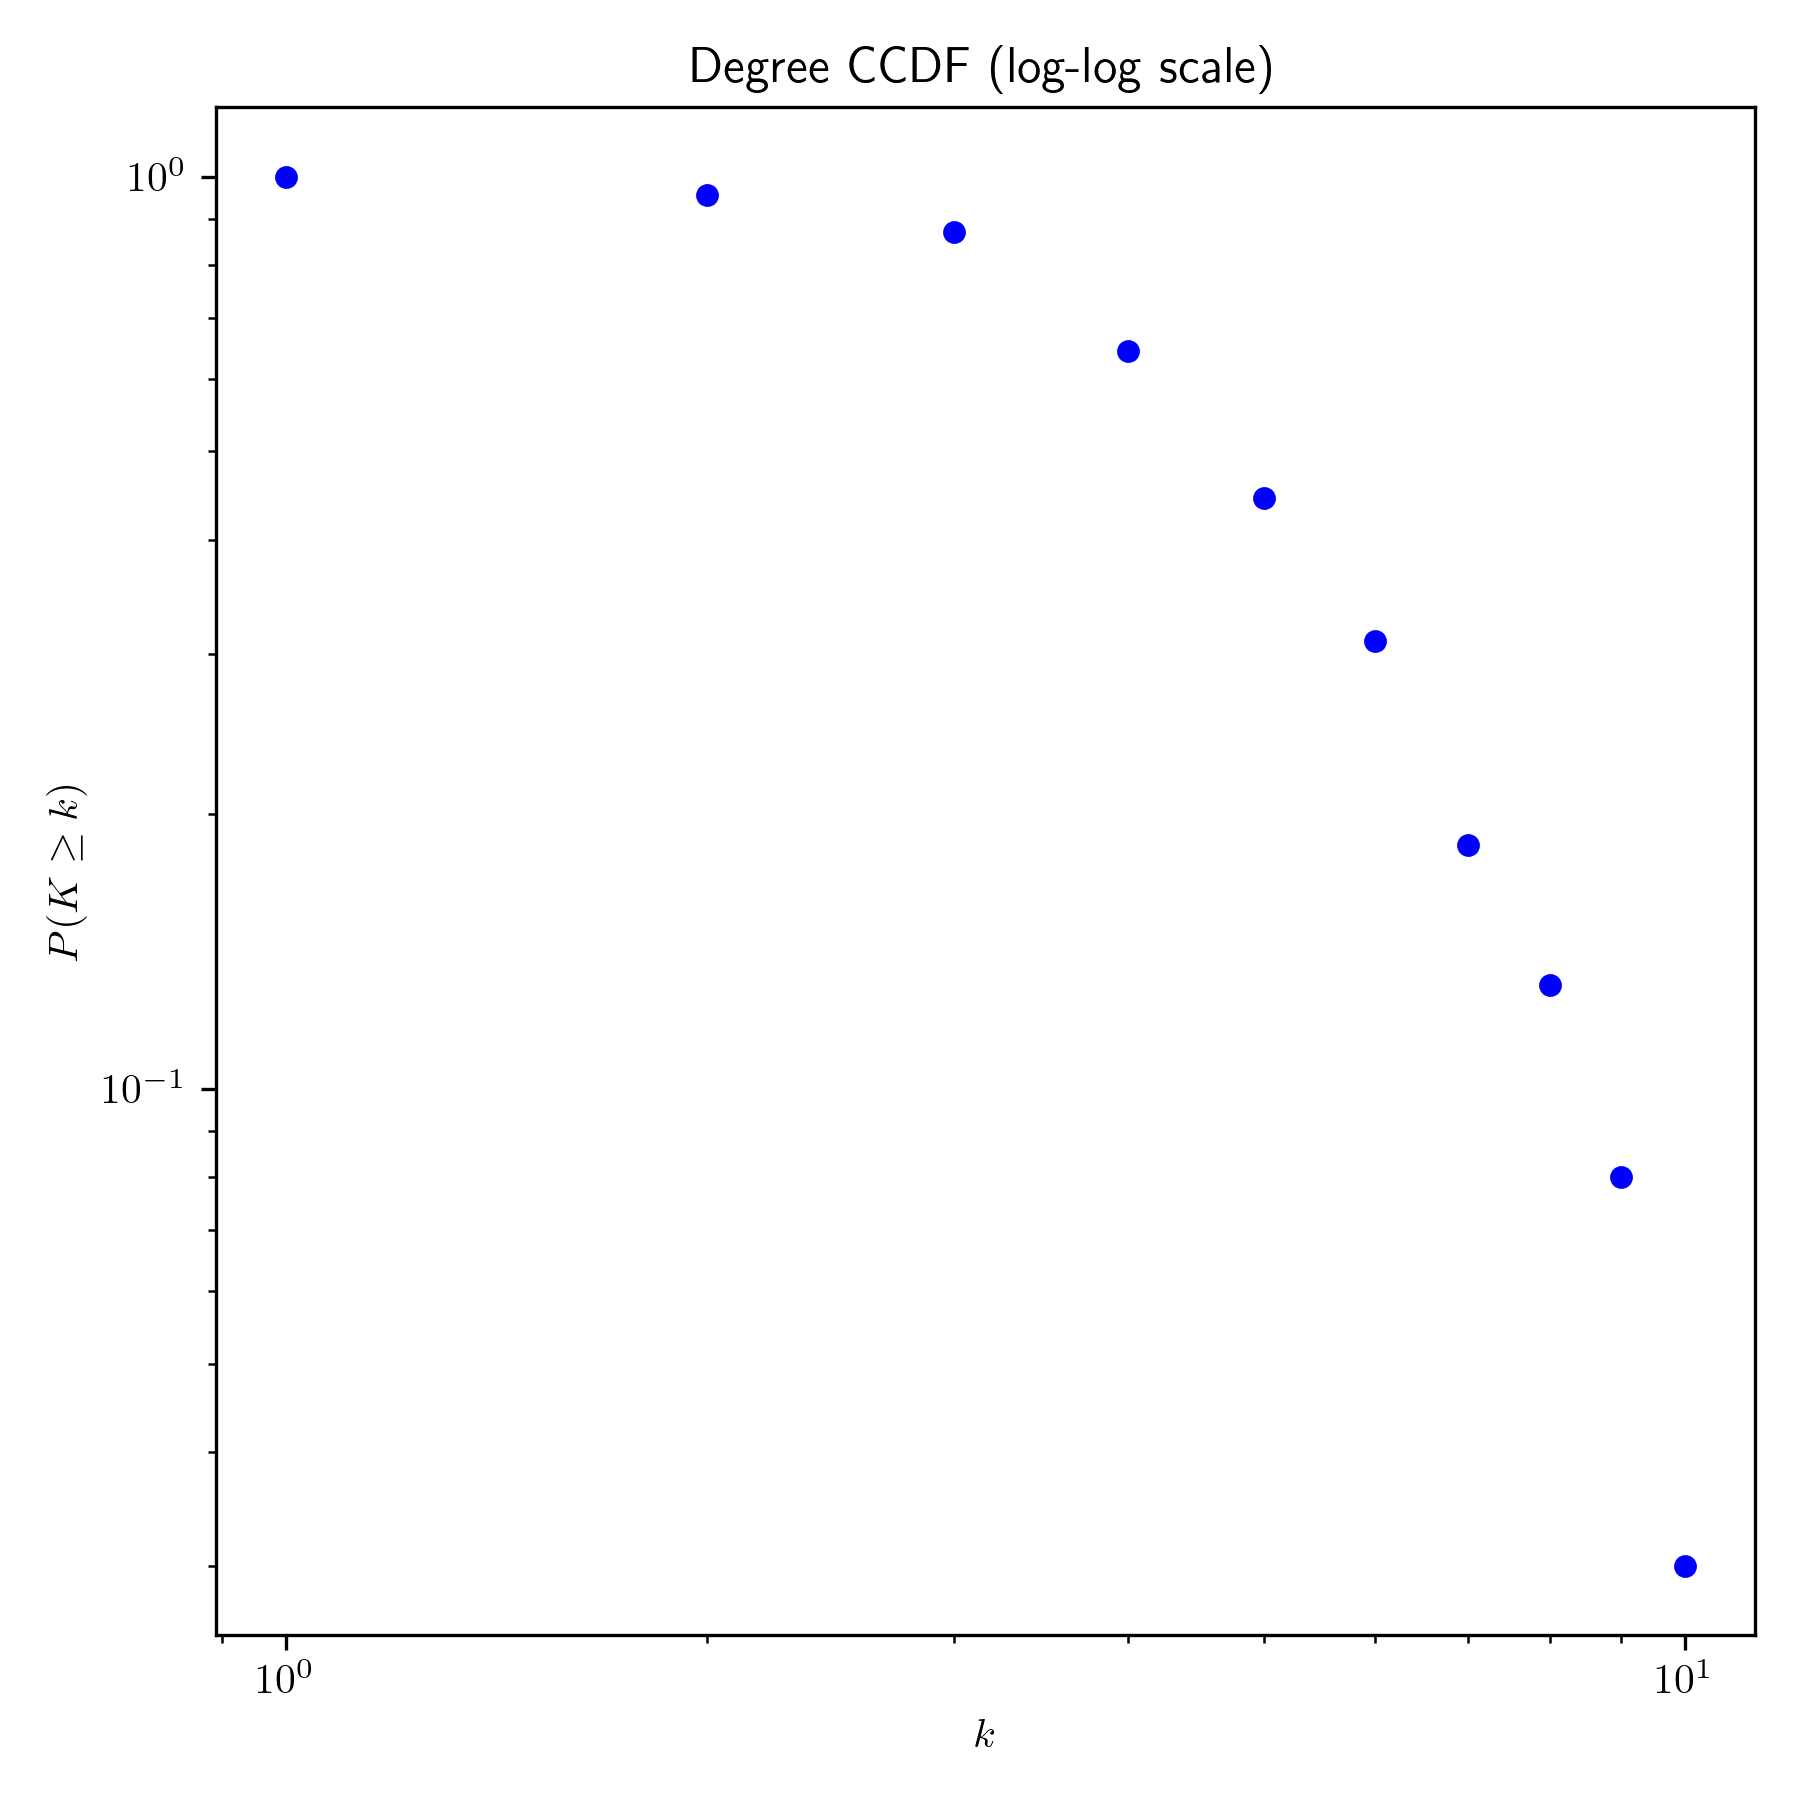
\includegraphics[width=0.8\textwidth]{assets/net5_ccdf.png}
        \caption{CCDF of the degree distribution of the complete network 5 in log-log space.}
    \end{subfigure}
    \caption{Degree distribution of the complete network 5. Left: histogram of the degree distribution. Right: CCDF of the degree distribution in log-log space. The degree distribution does not follow a power law, as the CCDF does not follow a straight line in log-log space.}
    \label{fig:net5_degree_distribution}
\end{figure}

The degree distribution shown in \Cref{fig:net5_degree_distribution} indicates that this network is not scale-free. In a scale-free network, the degree distribution follows a power law, which would appear approximately as a straight line in the CCDF represented in log-log space. This is clearly not the case here, since the curve bends. Moreover, the degree values are relatively limited, with a maximum degree of only 10 and an average degree of 4.4, which means that there are no hubs that characterize scale-free networks.

\begin{table}[h]
\centering
\begin{tabular}{lc}
\toprule
\textbf{Metric} & \textbf{net5} \\
\midrule
Number of nodes & 125 \\
Number of edges & 275 \\
Max degree & 10 \\
Min degree & 1 \\
Average degree & 4.4 \\
Avg. clustering coefficient & 0.5475 \\
Degree assortativity & 0.5373 \\
Avg. shortest path length & 13.131 \\
Diameter & 35 \\
\bottomrule
\end{tabular}
\caption{Structural characterization of the largest connected component of the net5 network.}
\label{tab:network5_characterization}
\end{table}

The largest connected component is also not a small-world network. Quantitatively, although the clustering coefficient is high (0.5475), both $\langle l\rangle$ (13.131) and the diameter (35) are too large for a connected component of only 125 nodes (see \Cref{tab:network5_characterization}). A small-world network is expected to combine high clustering with short path lengths, but here the distances between nodes remain large, indicating that many intermediate nodes have to be traversed to move across the network. Therefore, the network does not satisfy the defining combination of properties of the small-world phenomenon.

This conclusion is also supported qualitatively by the visualization of the largest connected component in \Cref{fig:extra_network_lcc}. It can be seen how there are many short connections between nearby nodes, but almost no long-range shortcuts linking distant parts of the component through hub nodes.

Overall, the combination of disconnected components in the full graph, the non-scale-free degree distribution, the high clustering, the high assortativity (0.5373), and the large path lengths strongly suggests that this extra network has been generated by a spatial model.

One of the simplest spatial models is the random geometric graph (RGG)~\cite{penrose2003random}. This model generates a network by placing $N$ nodes uniformly at random in a metric space (often a unit square) and connecting pairs of nodes that are within a certain distance $r$ of each other. The lower the value of $r$, the more likely it is that the resulting graph will be disconnected, as nodes that are far apart will not be connected. As $r$ increases, the graph becomes more connected, and for sufficiently large $r$, it will almost surely become fully connected.

We have implemented a RGG model. However, exactly reproducing a network with the same structural properties using only the number of nodes would be difficult, due to the randomness in the spatial placement of nodes. Different realizations of node positions can lead to significantly different network structures, even with the same values of $N$ and radius $r$. Nevertheless, since the positions of the nodes in this network are available, a more controlled approach is to generate RGGs using these fixed positions and see how the network structure evolves as a function of $r$. Having access to the node positions allows to calculate the value of $r$ beforehand, as the maximum distance between any pair of nodes is known.
\begin{equation}\label{eq:radius}
    r = \max_{i,j} d(i,j),
\end{equation}
where $d(i,j)$ is the distance between nodes $i$ and $j$. We assume that the distance between nodes is calculated using the Euclidean distance. Using \Cref{eq:radius}, a value of $r=0.09$ is obtained.

\begin{figure}[htbpt]
    \centering
    \begin{subfigure}[b]{0.31\textwidth}
        \centering
        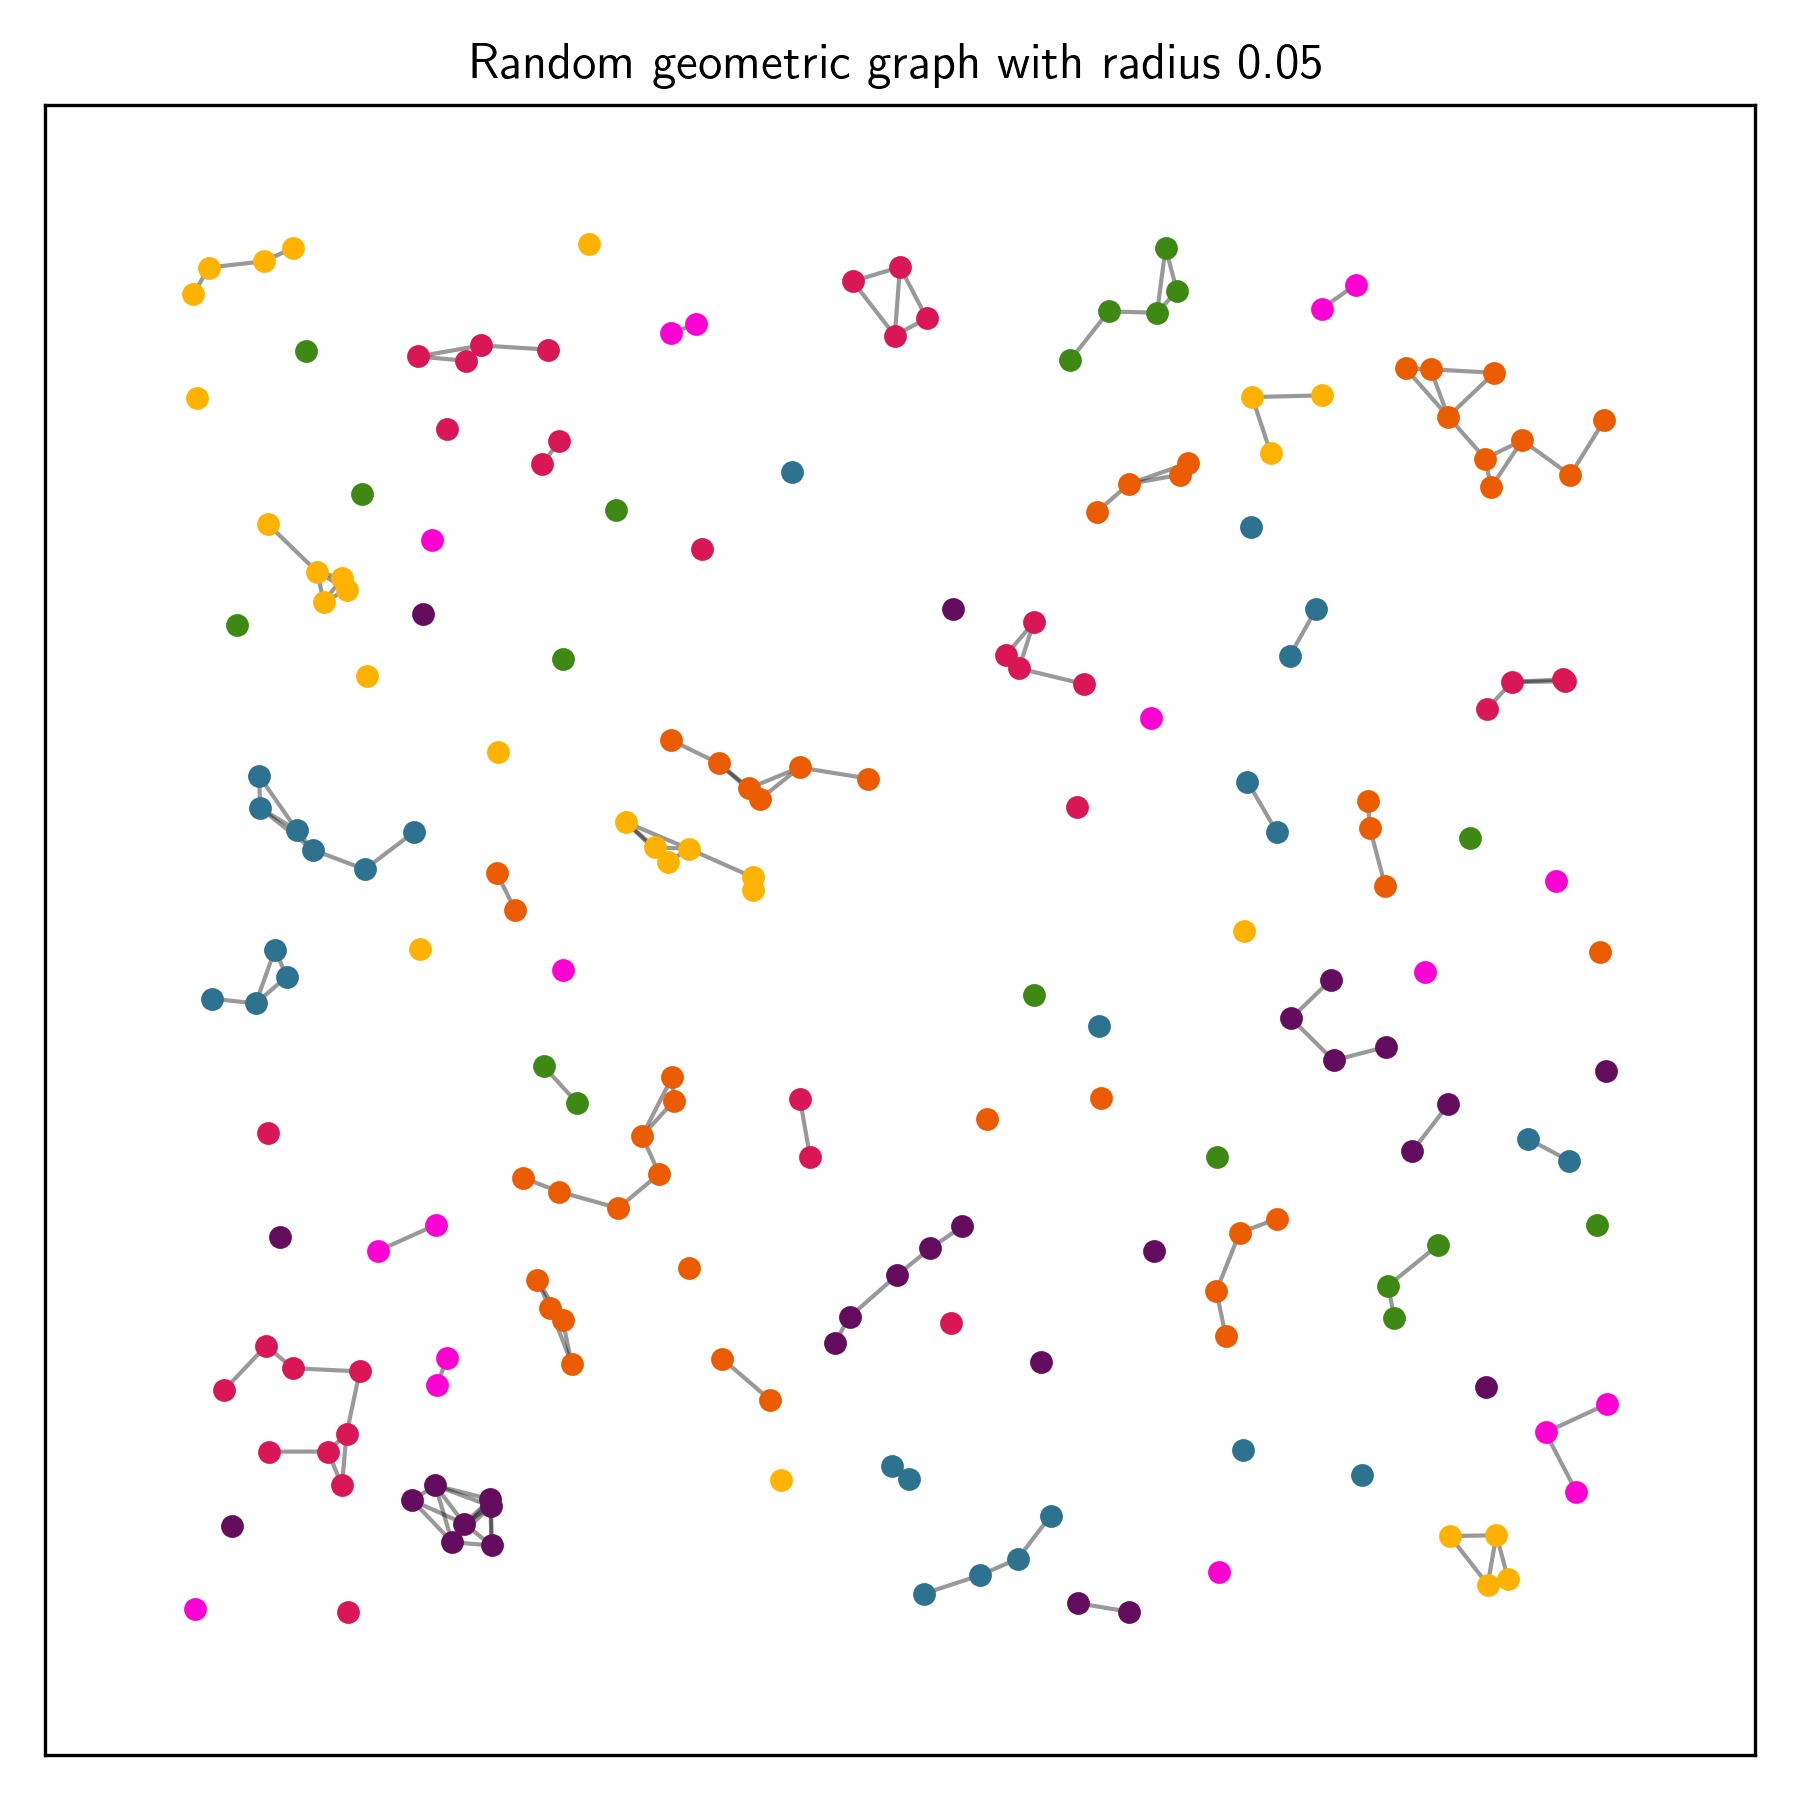
\includegraphics[width=\textwidth]{assets/net5_rgg_0.05.png}
        \caption{$r=0.05$}
        \label{fig:rgg_r005}
    \end{subfigure}\hfill
    \begin{subfigure}[b]{0.31\textwidth}
        \centering
        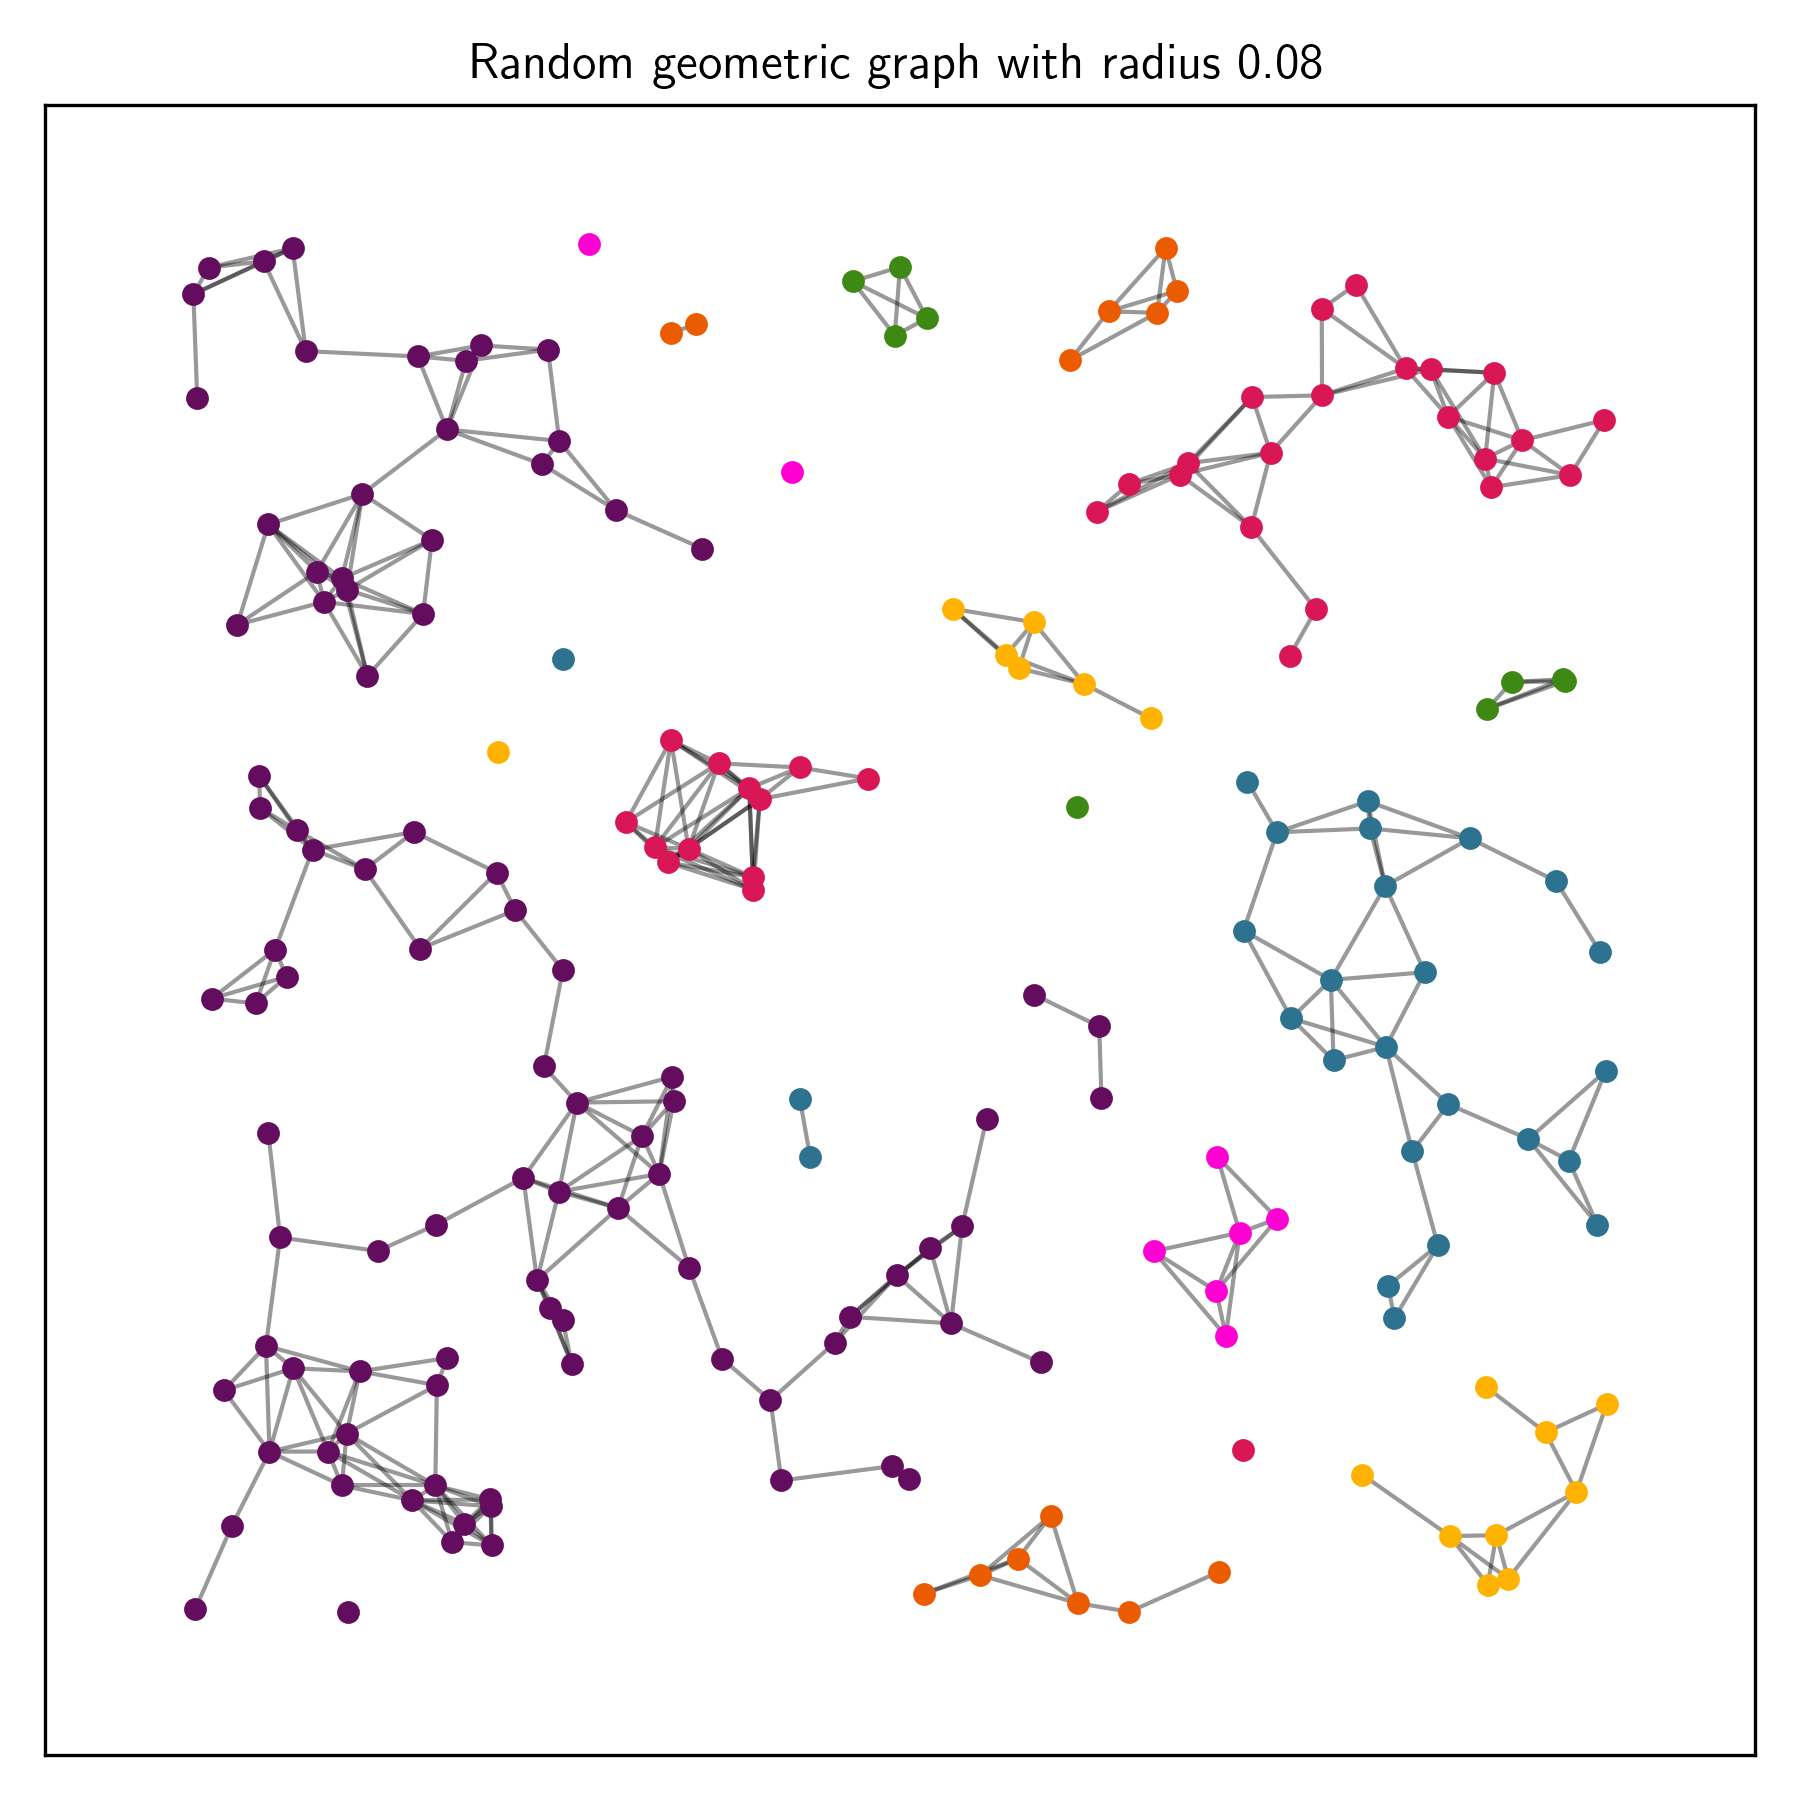
\includegraphics[width=\textwidth]{assets/net5_rgg_0.08.png}
        \caption{$r=0.08$}
        \label{fig:rgg_r008}
    \end{subfigure}\hfill
    \begin{subfigure}[b]{0.31\textwidth}
        \centering
        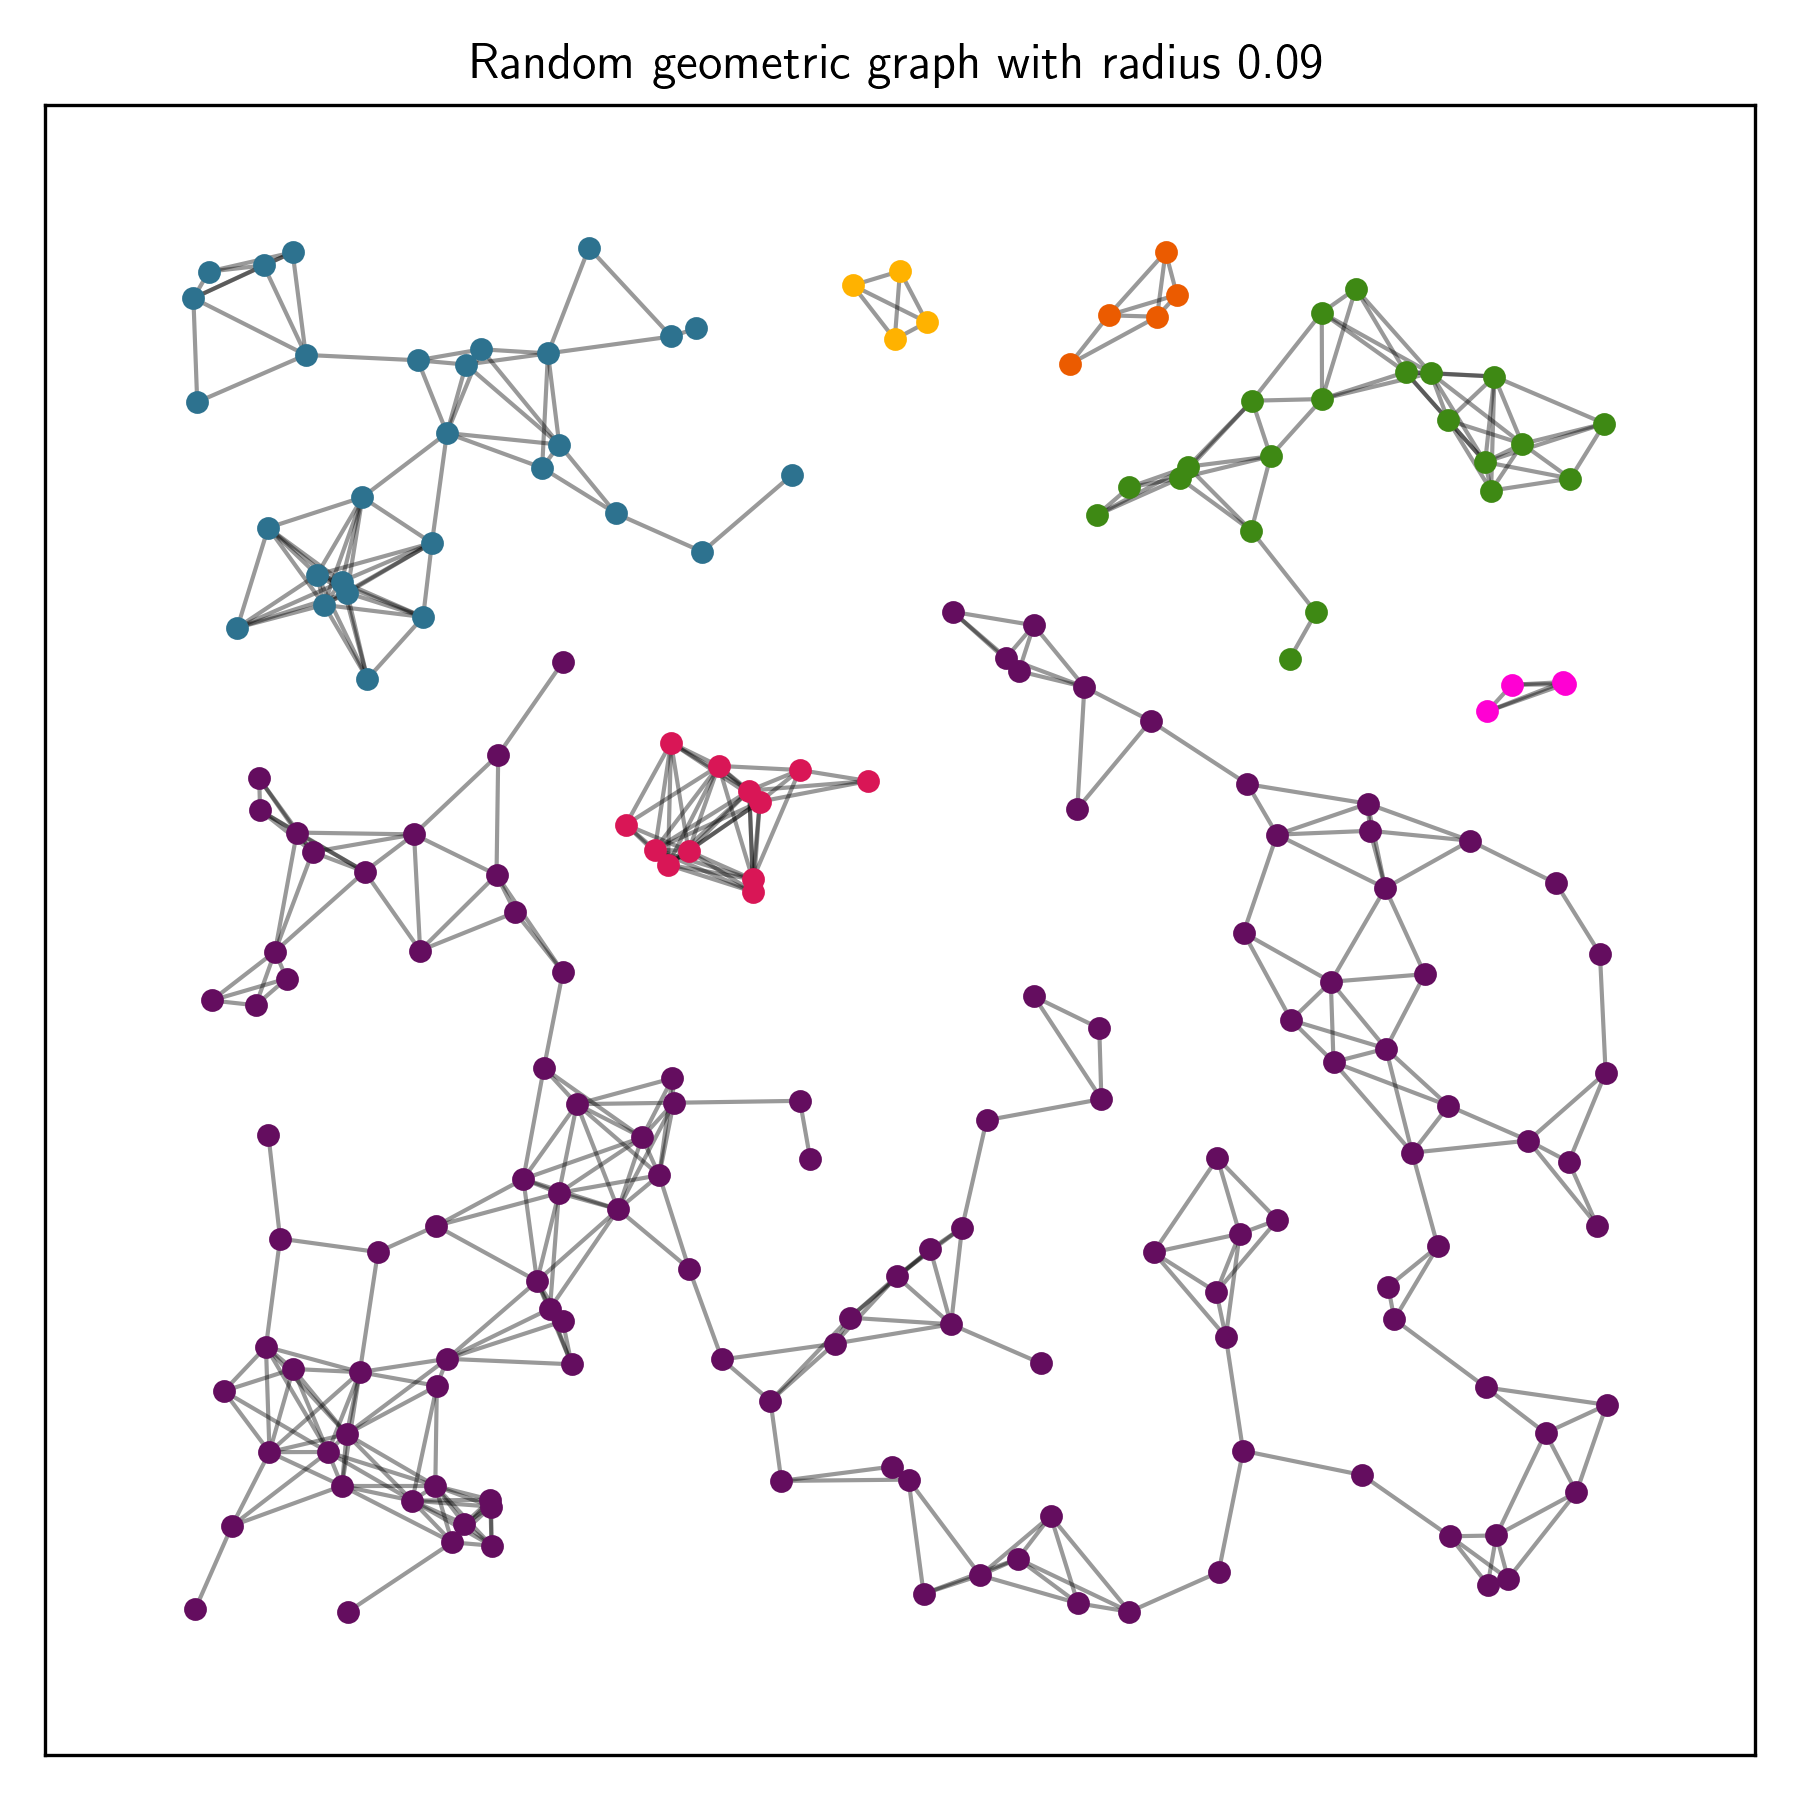
\includegraphics[width=\textwidth]{assets/net5_rgg_0.09.png}
        \caption{$r=0.09$}
        \label{fig:rgg_r009}
    \end{subfigure}

    \vspace{0.6em}

    \begin{subfigure}[b]{0.31\textwidth}
        \centering
        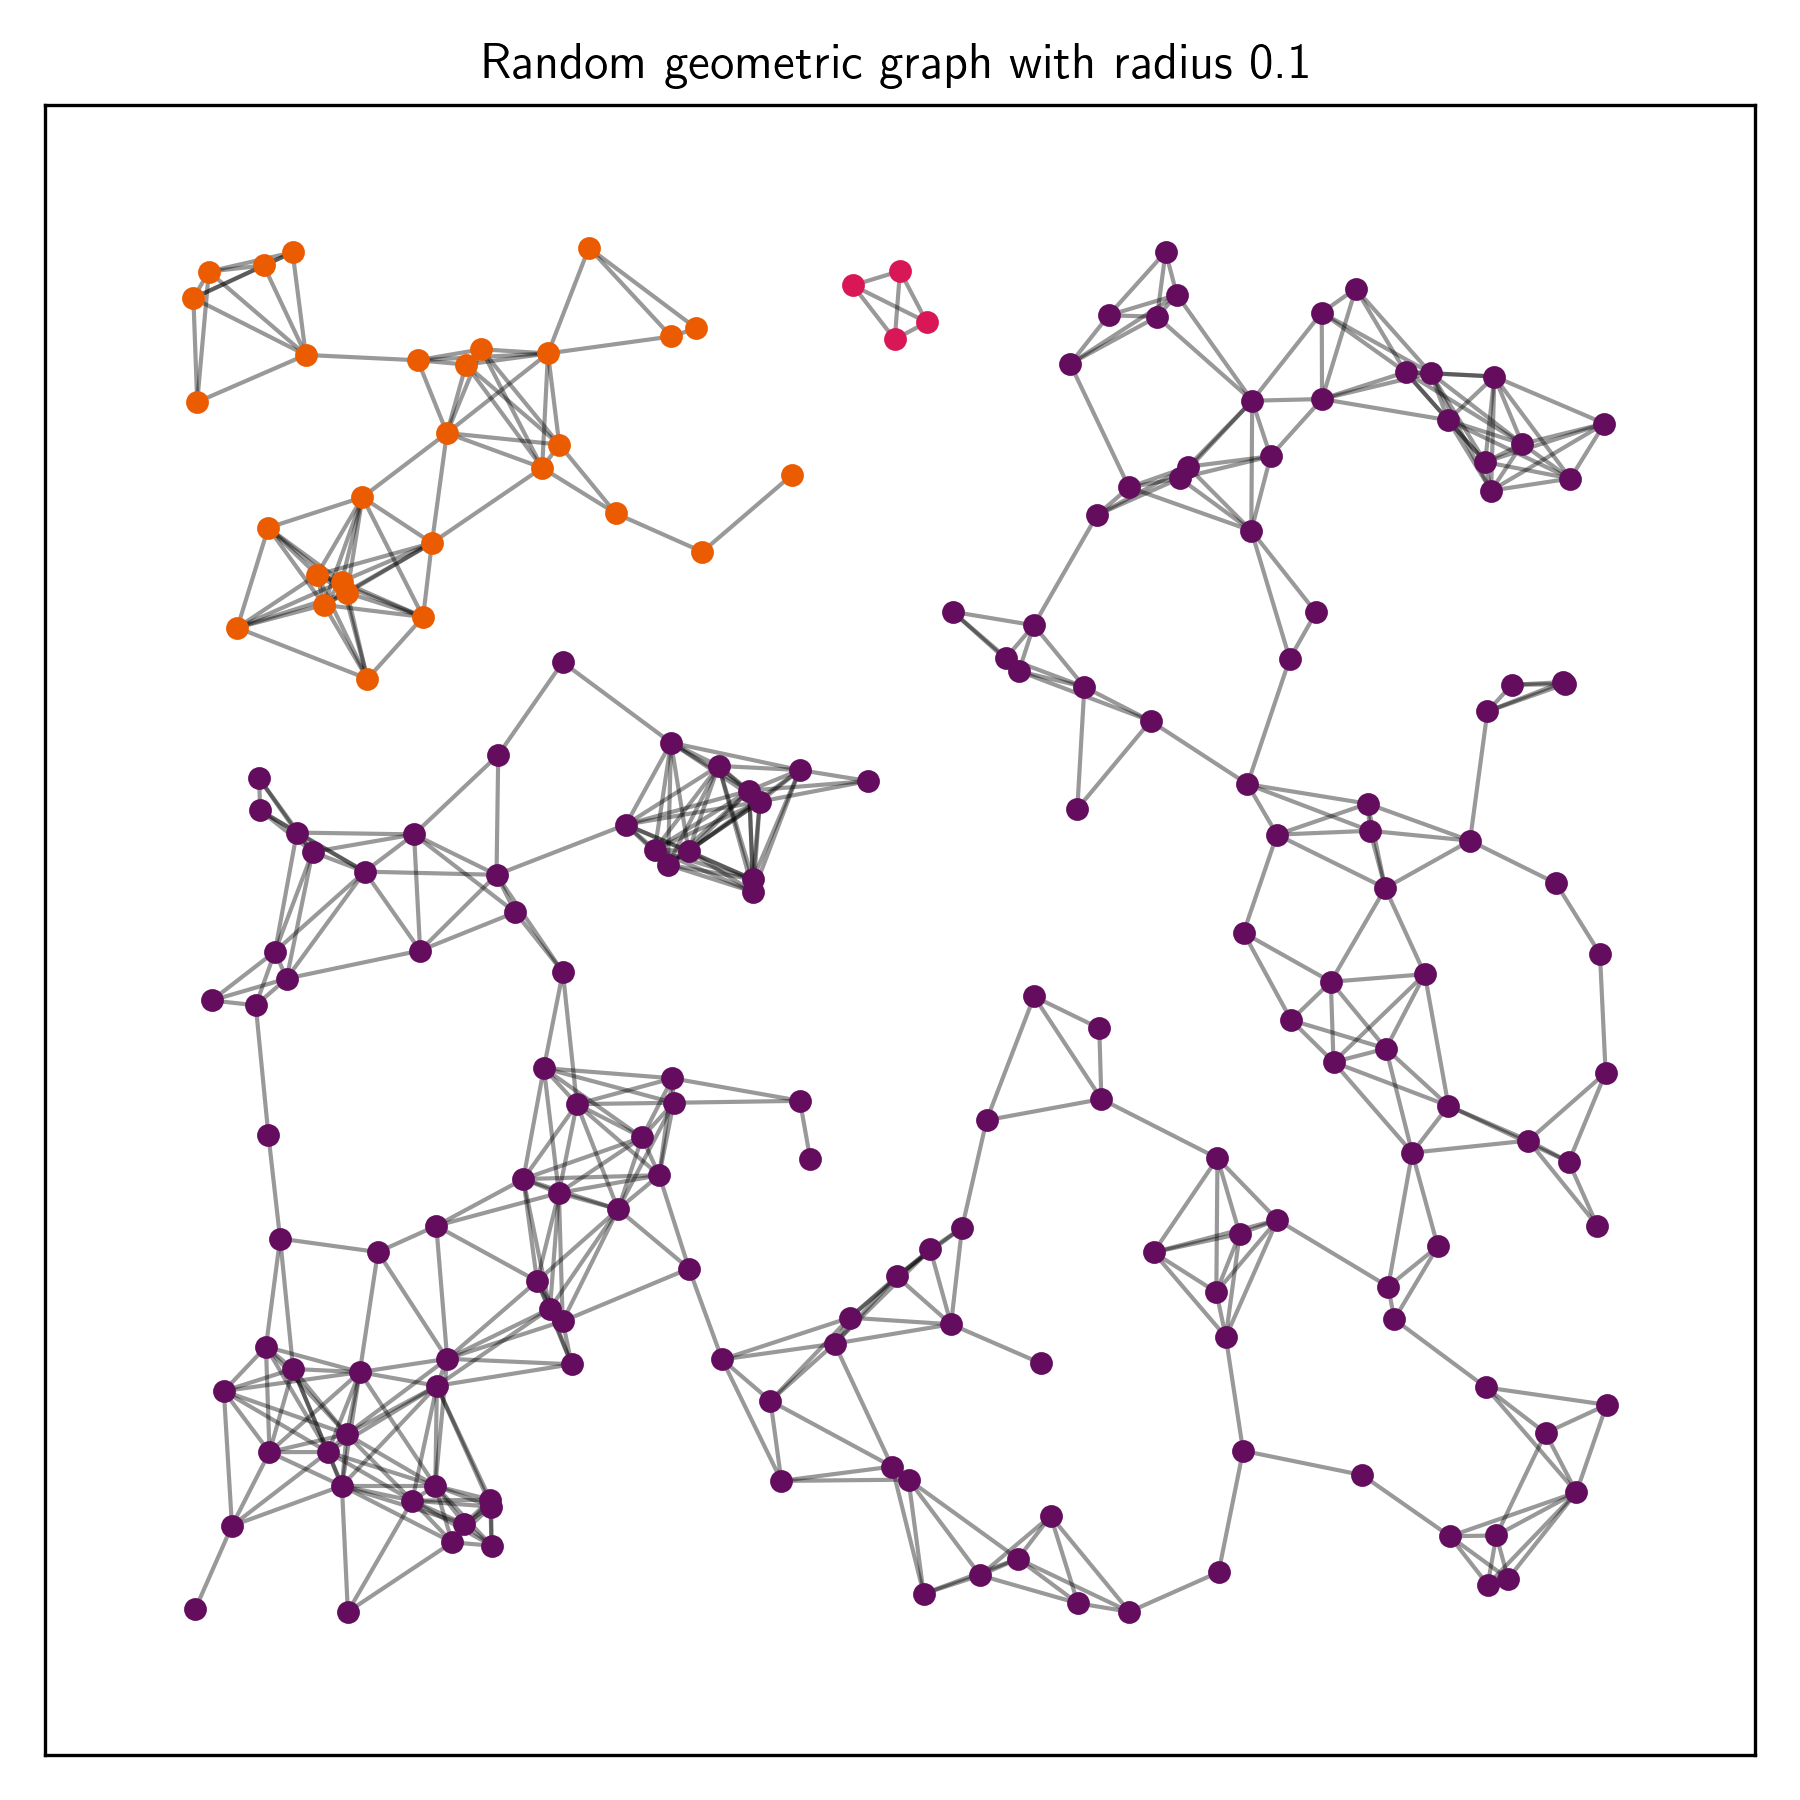
\includegraphics[width=\textwidth]{assets/net5_rgg_0.1.png}
        \caption{$r=0.10$}
        \label{fig:rgg_r010}
    \end{subfigure}\hfill
    \begin{subfigure}[b]{0.31\textwidth}
        \centering
        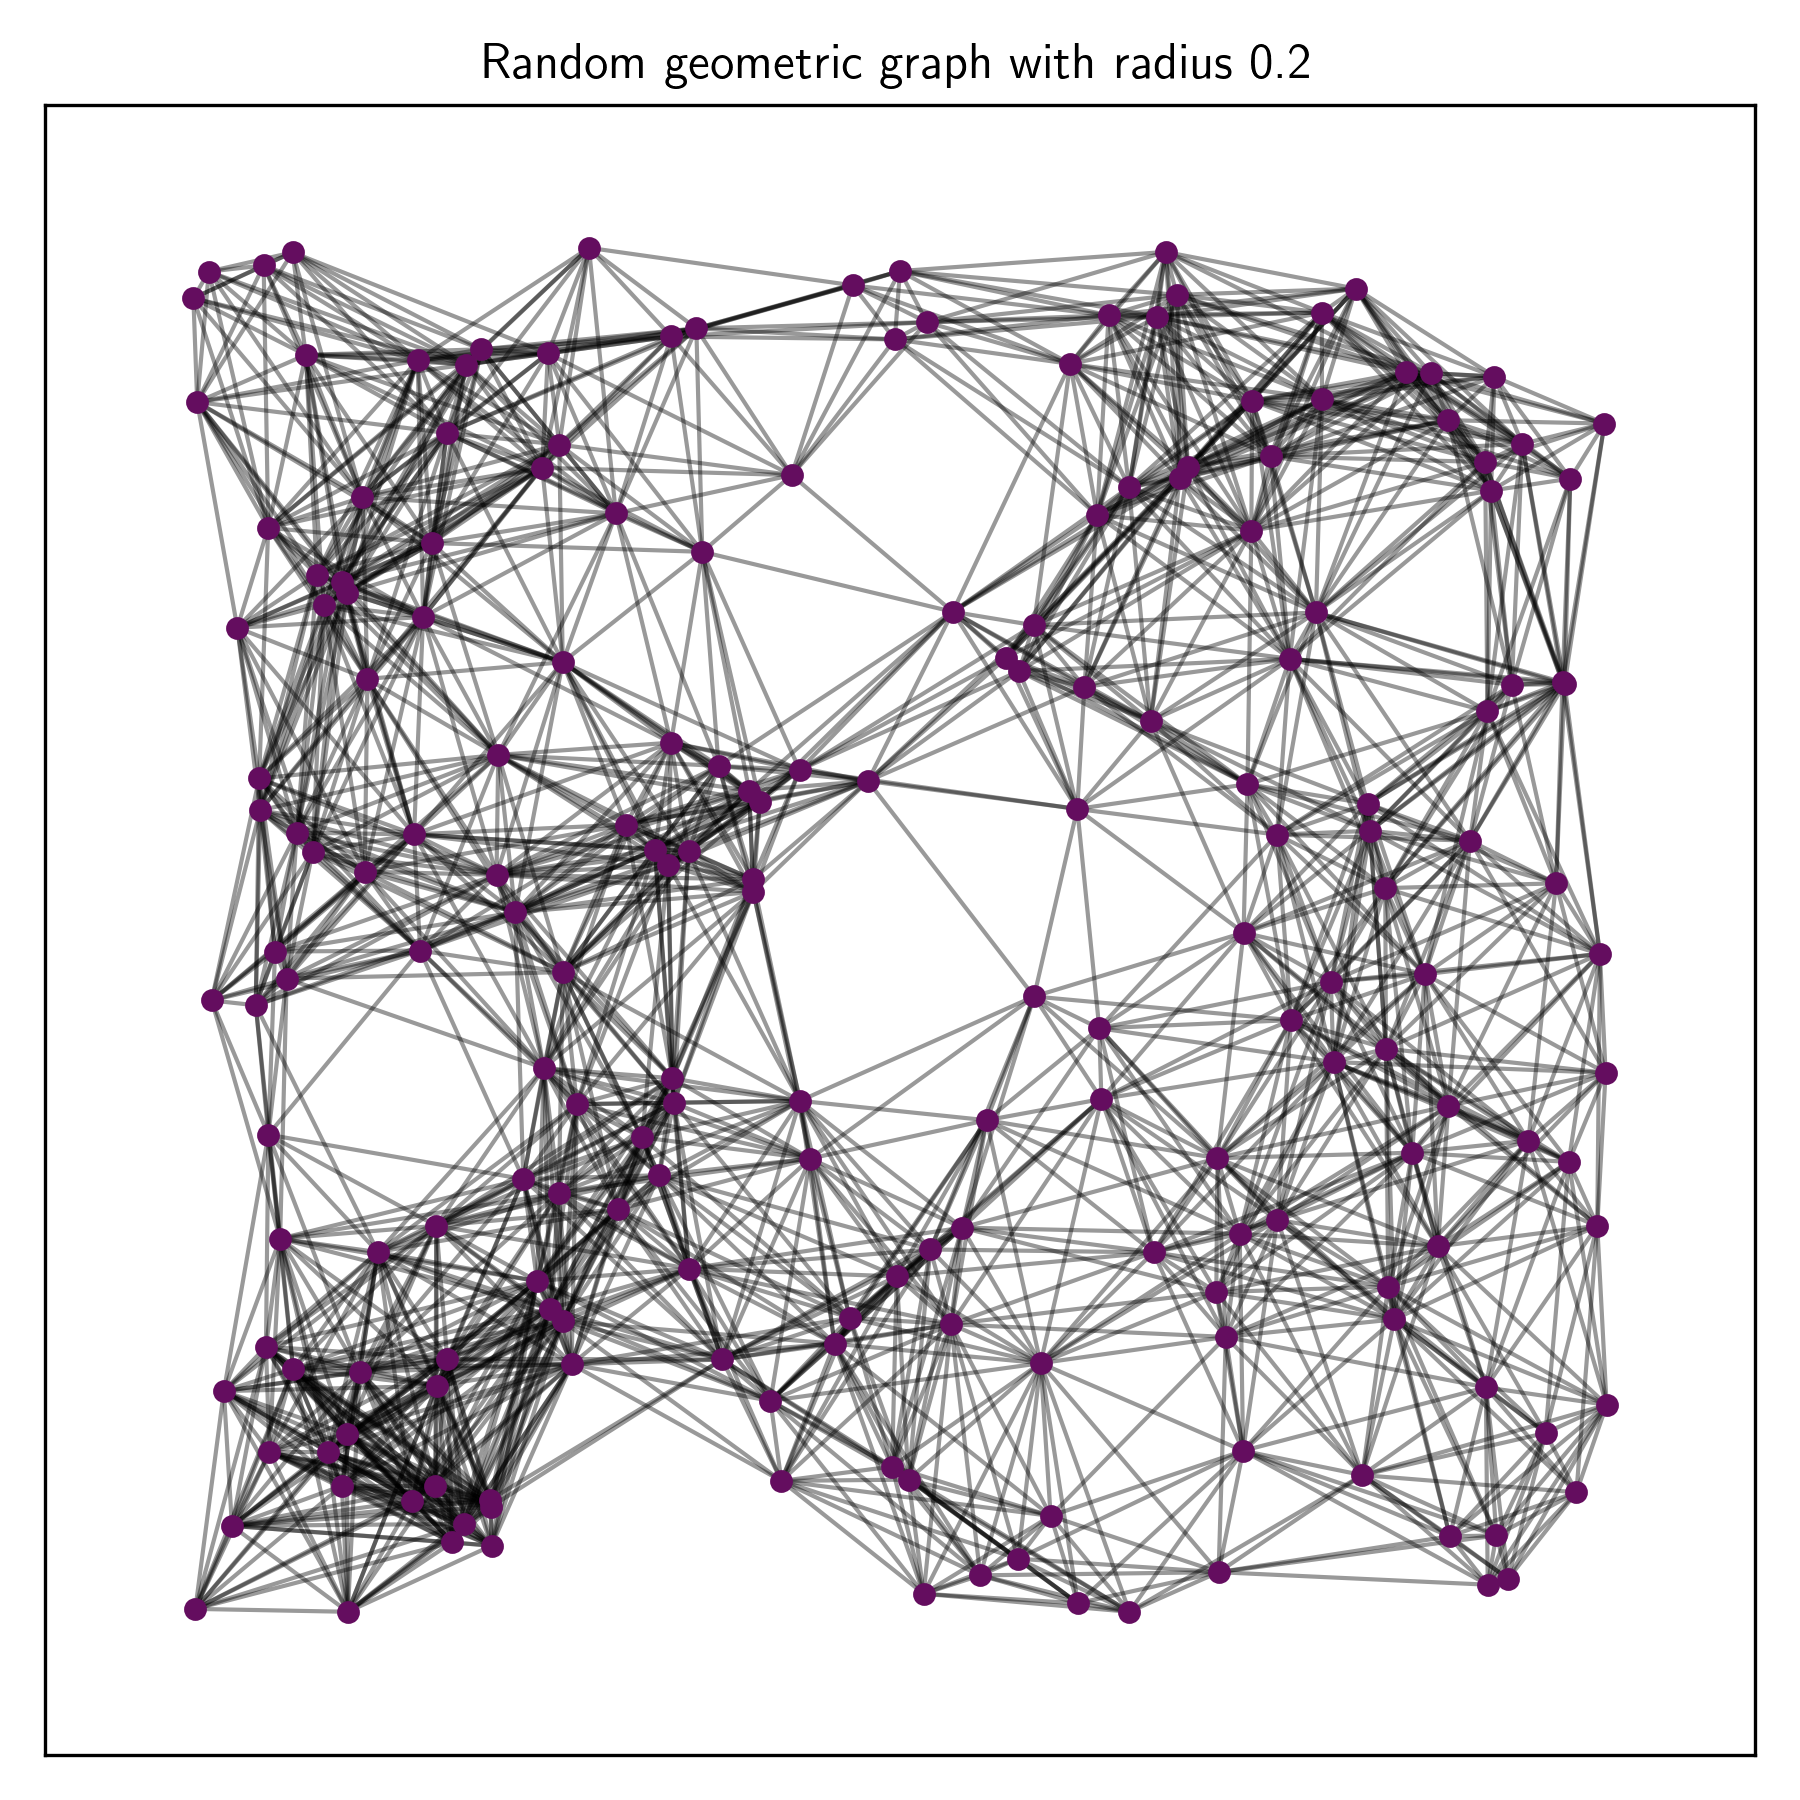
\includegraphics[width=\textwidth]{assets/net5_rgg_0.2.png}
        \caption{$r=0.20$}
        \label{fig:rgg_r020}
    \end{subfigure}
    \caption{Random geometric graphs generated from the same node positions for different values of the connection radius $r$.}
    \label{fig:rgg_radius_sweep}
\end{figure}

\Cref{fig:rgg_radius_sweep} shows the expected transition as $r$ increases. For small radius (e.g., $r=0.05$), the graph is highly fragmented because only very close nodes are connected. As $r$ grows ($r=0.08$ and $r=0.09$), local clusters start to merge and the global structure becomes similar to the observed extra network. For larger radius ($r=0.10$ and especially $r=0.20$), many additional links appear and the network becomes much denser than the original one. This confirms that using $r=0.09$ indeed reproduces the original network.




\section{Conclusions}

In this report, we have shown how the structural descriptors provide powerful tools for understanding the organization of complex networks. By combining macroscopic and microscopic analyses, we have been able to distinguish between homogeneous and heterogeneous topologies, identify the presence of hubs, and evaluate the small-world properties. We have associated each network with its corresponding generative model, and the simulations generated suggest that these models have been correctly matched to their respective networks.

For the fifth network, a different approach has been followed, leading to the exploration of a model not covered in the theoretical lectures. In particular, a spatial model based on node positions has been proposed as a possible mechanism to generate the network.

\newpage
\bibliography{references}

\clearpage

% \appendix

% \section{Rule definition prompt}\label{sec:prompt}
% This section includes the prompt used to generate the initial set of rules for our fuzzy expert system using DeepSeek.
% \lstinputlisting{prompt.txt}

\end{document}
